\documentclass[aspectratio=169, 10pt]{beamer}

% Modern Font and Math Packages
\usepackage{amsmath, amssymb, amsfonts}
\usepackage{booktabs}
\usepackage{graphicx}
\usepackage{tikz}
\usepackage{tcolorbox}
\usepackage{microtype}
\usepackage{hyperref}
\tcbuselibrary{skins}

% Color Palette - Clean Academic Light (Navy & Royal Slate)
\definecolor{PrimaryNavy}{RGB}{10, 37, 64}      % Deep Navy
\definecolor{AccentBlue}{RGB}{0, 102, 204}     % Royal Vivid Blue
\definecolor{DarkSlate}{RGB}{45, 55, 72}       % Dark Slate Charcoal
\definecolor{LightGreyBg}{RGB}{247, 250, 252}  % Subtle Off-White Card Fill
\definecolor{BorderGrey}{RGB}{226, 232, 240}   % Crisp Card Border
\definecolor{EmeraldGreen}{RGB}{16, 185, 129}  % KPI Success Accent
\definecolor{AlertRed}{RGB}{225, 29, 72}       % Alert Accent

% Beamer Global Theme Settings
\setbeamercolor{background canvas}{bg=white}
\setbeamercolor{normal text}{fg=DarkSlate}
\setbeamercolor{frametitle}{fg=PrimaryNavy, bg=white}
\setbeamercolor{title}{fg=PrimaryNavy}
\setbeamercolor{subtitle}{fg=AccentBlue}
\setbeamercolor{author}{fg=DarkSlate}
\setbeamercolor{institute}{fg=DarkSlate!80}
\setbeamercolor{date}{fg=DarkSlate!70}

% Turn off default navigation symbols
\setbeamertemplate{navigation symbols}{}

% Custom Frametitle Formatting
\setbeamertemplate{frametitle}{
    \vspace{0.25cm}
    {\large\bfseries\color{PrimaryNavy}\insertframetitle}
    \ifx\insertframesubtitle\empty\else
        \\[-0.1cm]{\scriptsize\color{AccentBlue}\textbf{\insertframesubtitle}}
    \fi
    \vspace{0.08cm}
    \hrule height 0.6pt \color{BorderGrey}
}

% Custom Footline - Modern Technical Style
\setbeamertemplate{footline}{
    \leavevmode%
    \begin{tikzpicture}[remember picture, overlay]
        \draw[BorderGrey, line width=0.45pt] ([yshift=0.55cm]current page.south west) -- ([yshift=0.55cm]current page.south east);
    \end{tikzpicture}%
    \hbox{%
        \begin{beamercolorbox}[wd=\paperwidth,ht=2.8ex,dp=1.2ex,leftskip=0.8cm,rightskip=0.8cm]{footline}
            {\tiny%
                \textbf{\color{PrimaryNavy}AI Academy} \textcolor{BorderGrey!150}{$\mid$} \textcolor{DarkSlate!85}{Group M001 $\cdot$ Team Qarabağ Zəfəri}%
                \hfill%
                \textbf{\color{AccentBlue}AZN-Vision: Assistive Banknote Intelligence}%
                \hfill%
                \textbf{\color{PrimaryNavy}\insertframenumber}\textcolor{DarkSlate!40}{~/~}\textbf{\color{DarkSlate!70}\inserttotalframenumber}%
            }%
        \end{beamercolorbox}%
    }%
    \vskip0pt%
}

% Custom tcolorbox Card Components
\newtcolorbox{card}[1]{
    enhanced,
    colback=LightGreyBg,
    colframe=BorderGrey,
    coltitle=PrimaryNavy,
    fonttitle=\bfseries\footnotesize,
    title=#1,
    arc=2mm,
    boxrule=0.75pt,
    left=5pt, right=5pt, top=3pt, bottom=3pt,
    boxsep=1pt,
    toptitle=1pt, bottomtitle=1pt
}

\newtcolorbox{techblock}[1]{
    enhanced,
    colback=white,
    colframe=AccentBlue,
    coltitle=white,
    colbacktitle=AccentBlue,
    fonttitle=\bfseries\footnotesize,
    title=#1,
    arc=2mm,
    boxrule=0.75pt,
    left=5pt, right=5pt, top=3pt, bottom=3pt,
    boxsep=1pt,
    toptitle=1pt, bottomtitle=1pt
}

\newtcolorbox{alertblockcustom}[1]{
    enhanced,
    colback=white,
    colframe=AlertRed,
    coltitle=white,
    colbacktitle=AlertRed,
    fonttitle=\bfseries\footnotesize,
    title=#1,
    arc=2mm,
    boxrule=0.75pt,
    left=5pt, right=5pt, top=3pt, bottom=3pt,
    boxsep=1pt,
    toptitle=1pt, bottomtitle=1pt
}

\newcommand{\kpitech}[3]{
    \begin{tcolorbox}[
        enhanced,
        colback=LightGreyBg,
        colframe=AccentBlue,
        arc=2mm,
        boxrule=1pt,
        left=3pt, right=3pt, top=3pt, bottom=3pt,
        halign=center
    ]
        {\small\bfseries\color{PrimaryNavy} #1}\\
        {\tiny\bfseries\color{AccentBlue} #2}\\
        {\tiny\color{DarkSlate!80} #3}
    \end{tcolorbox}
}

% Presentation Metadata
\title[AZN-Vision Defense]{\huge\textbf{AZN-Vision: Assistive Banknote Intelligence}}
\subtitle{\large Wearable Edge Vision System for the Visually Impaired}
\author[Team Qarabağ Zəfəri]{
    \textbf{Avaz Asgarov} \and \textbf{Kazim Mammadli} \and \textbf{Gulnar Babazade} \\[0.1cm]
    \textbf{Hasan Mammadov} \and \textbf{Nicat Alaskarli}
}
\institute[AI Academy]{
    \textbf{Cohort I 2026} · National Artificial Intelligence Center\\
    Course: Deep Learning (DLE-AI-202) · Group: \textbf{M001}\\
    Team: \textbf{Qarabağ Zəfəri}
}
\date{Oral Defense · 13 September 2026}

\begin{document}

% ------------------------------------------------------------------------------
% ------------------------------------------------------------------------------
% Title Slide: Monumental Academic Defense Design
% ------------------------------------------------------------------------------
\begin{frame}[plain]
    \begin{tikzpicture}[remember picture, overlay]
        % Background geometric watermark (drawn first so it renders behind the navy header)
        \draw[BorderGrey!60, line width=1.5pt] ([xshift=-2.5cm, yshift=-2.5cm]current page.north east) circle (4.5cm);
        \draw[BorderGrey!40, line width=0.8pt] ([xshift=-2.5cm, yshift=-2.5cm]current page.north east) circle (5.5cm);

        % Deep Navy Top Header Banner (drawn on top of the watermark circles)
        \fill[PrimaryNavy] (current page.north west) rectangle ([yshift=-1.3cm]current page.north east);
        \node[anchor=west, text=white, font=\scriptsize\bfseries] at ([xshift=0.8cm, yshift=-0.65cm]current page.north west) {AI ACADEMY $\cdot$ NATIONAL ARTIFICIAL INTELLIGENCE CENTER};
        \node[anchor=east, text=white!85, font=\scriptsize\bfseries] at ([xshift=-0.8cm, yshift=-0.65cm]current page.north east) {COHORT I $\cdot$ CAPSTONE DEFENSE};

        % Subtle decorative accent line
        \fill[AccentBlue] ([yshift=-1.3cm]current page.north west) rectangle ([yshift=-1.36cm]current page.north east);
    \end{tikzpicture}
    
    \vspace{0.75cm}
    \begin{center}
        {\fontsize{21pt}{25pt}\selectfont\bfseries\color{PrimaryNavy} AZN-Vision: Assistive Banknote Intelligence}\\[0.20cm]
        {\small\bfseries\color{AccentBlue} Wearable Edge Vision System \& Micro-Architecture for the Visually Impaired}\\[0.15cm]
        {\tiny\color{DarkSlate!70}\textbf{Course: Deep Learning (DLE-AI-202) $\cdot$ Group: M001 $\cdot$ 13 September 2026}}
    \end{center}

    \vspace{0.20cm}
    \begin{columns}[c]
        \begin{column}{0.48\textwidth}
            \begin{techblock}{Engineering Team: Qarabağ Zəfəri}
                \small
                \begin{itemize}\setlength{\itemsep}{4pt}
                    \item \textbf{Avaz Asgarov}
                    \item \textbf{Kazim Mammadli}
                    \item \textbf{Gulnar Babazade}
                    \item \textbf{Hasan Mammadov}
                    \item \textbf{Nicat Alaskarli}
                \end{itemize}
            \end{techblock}
        \end{column}
        
        \begin{column}{0.48\textwidth}
            \begin{techblock}{Project Repository \& Codebase}
                \vspace{0.15cm}
                \centering
                {\footnotesize\bfseries\color{PrimaryNavy} Official Open-Source Implementation}\\[0.22cm]
                \href{https://github.com/AvazAsgarov/azerbaijani-banknote-vision}{%
                    \color{AccentBlue}\bfseries\small%
                    \underline{\texttt{github.com/AvazAsgarov/}}\\[0.08cm]%
                    \underline{\texttt{azerbaijani-banknote-vision}}%
                }\\[0.28cm]
                {\scriptsize\color{DarkSlate!85}\textbf{Public Engineering Artifacts:}}\\[0.08cm]
                {\tiny\color{DarkSlate!75} Deep Learning Models $\cdot$ ESP32-S3 Firmware $\cdot$ iOS App $\cdot$ Benchmark Audits}
                \vspace{0.15cm}
            \end{techblock}
        \end{column}
    \end{columns}
\end{frame}

% ------------------------------------------------------------------------------
% Modular Section Inclusions
% ------------------------------------------------------------------------------
% ==============================================================================
% SECTION 01: CURATED DOMAIN DATASET & SPLIT INTEGRITY
% AZN-Vision: Assistive Azerbaijani Banknote Recognition System
% Cohort I 2026 - AI Academy - National Artificial Intelligence Center
% Group: M001 | Team: Qarabağ Zəfəri
% ==============================================================================

% ------------------------------------------------------------------------------
% Slide 1 (Page 2): Domain Data Acquisition & Multi-Annotator Protocol
% ------------------------------------------------------------------------------
\begin{frame}{Domain Data Acquisition \& Multi-Annotator Protocol}{Gold-Standard Ground Truth with Proven Inter-Annotator Agreement}
    \begin{columns}[c]
        \begin{column}{0.54\textwidth}
            \begin{techblock}{In-the-Wild Numismatic Capture}
                \footnotesize
                \begin{itemize}\setlength{\itemsep}{2pt}
                    \item \textbf{Scope:} 7 circulating AZN notes (1 to 200 AZN).
                    \item \textbf{Raw Ingestion:} 2,593 captures across 93 unconstrained scenes.
                    \item \textbf{Data Hygiene:} 71 frames pruned (52 duplicates, 19 empty labels).
                    \item \textbf{Production Benchmark:} \textbf{2,522 active unique notes}.
                \end{itemize}
            \end{techblock}
            
            \vspace{0.12cm}
            \begin{alertblockcustom}{Multi-Annotator Calibration Protocol}
                \footnotesize
                \begin{itemize}\setlength{\itemsep}{2pt}
                    \item \textbf{Calibration Protocol:} 5 annotators on 150 benchmark images.
                    \item \textbf{Spatial IoU Agreement:} \textbf{93.4\%} ($\pm 0.028$, median: 94.8\%).
                    \item \textbf{Label Concordance:} \textbf{98.8\%} (Fleiss' $\kappa = 0.962$).
                \end{itemize}
            \end{alertblockcustom}
        \end{column}
        
        \begin{column}{0.44\textwidth}
            \begin{card}{Dataset Breakdown (2522 Clean Notes)}
                \centering
                \scriptsize
                \renewcommand{\arraystretch}{1.05}
                \begin{tabular}{l l r}
                    \toprule
                    \textbf{Denom} & \textbf{Numismatic Motif} & \textbf{Count} \\
                    \midrule
                    \textbf{001 AZN} & Tar \& Folk Culture & 439 \\
                    \textbf{005 AZN} & Literature \& Poetry & 297 \\
                    \textbf{010 AZN} & Old City Architecture & 493 \\
                    \textbf{020 AZN} & Military \& Karabakh & 314 \\
                    \textbf{050 AZN} & Education \& Youth & 321 \\
                    \textbf{100 AZN} & Modern Infrastructure & 377 \\
                    \textbf{200 AZN} & Modernist Architecture & 281 \\
                    \bottomrule
                \end{tabular}
            \end{card}
            
            \vspace{0.12cm}
            \kpitech{93.4\% Mean IoU}{5-Member Blinded Agreement Calibration}{Fleiss' $\kappa = 0.962$ verifies robust mutual ground truth}
        \end{column}
    \end{columns}
\end{frame}

% ------------------------------------------------------------------------------
% Slide 2 (Page 3): In-the-Wild Dataset Visual Showcase (Batch Sample Grid)
% ------------------------------------------------------------------------------
\begin{frame}{Authentic Numismatic Spectrum}{Real-World Capture Diversity Across All Circulating Denominations}
    \centering
    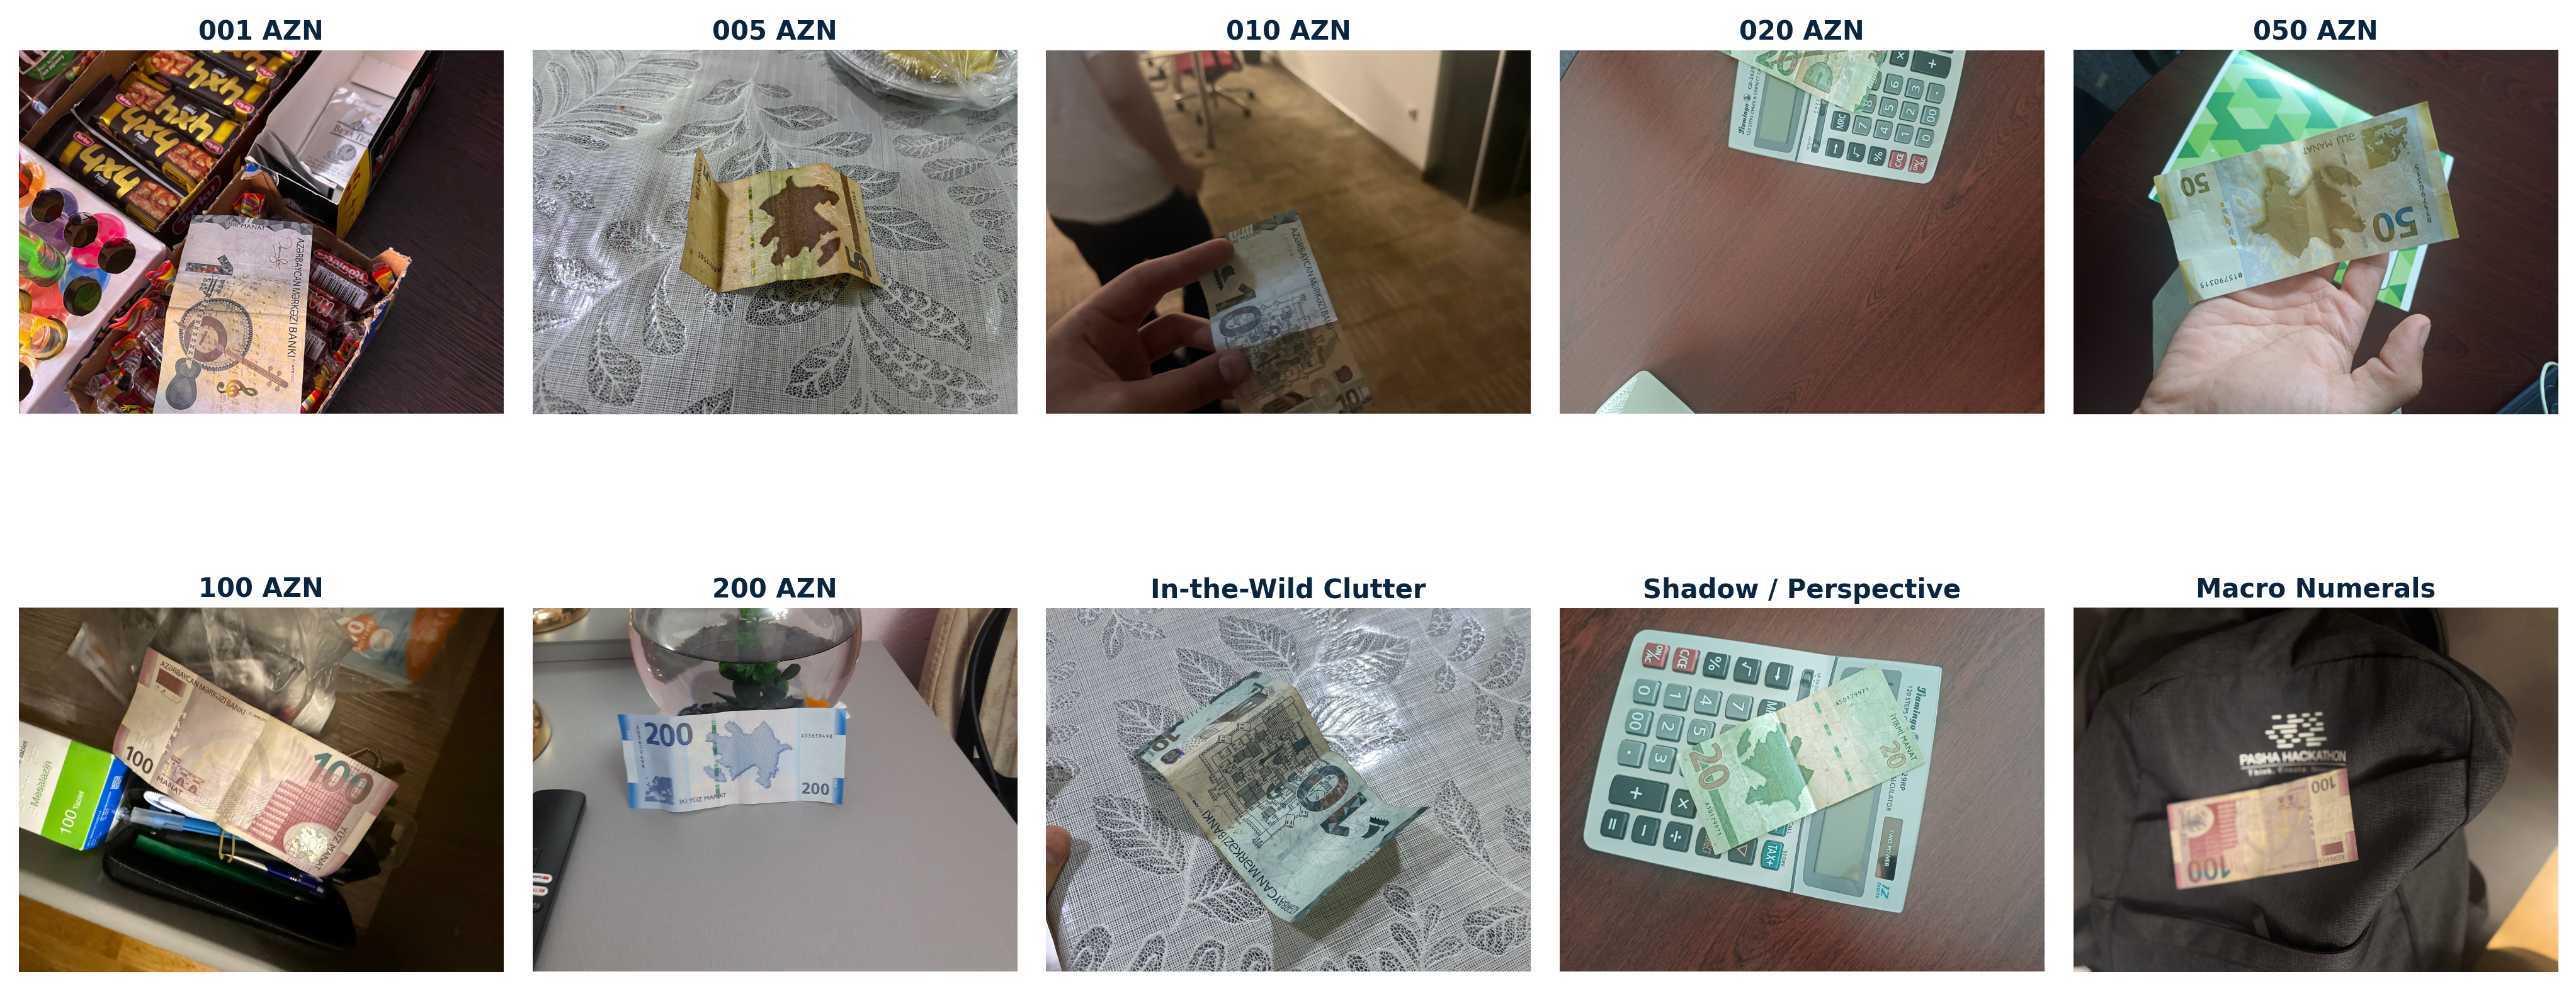
\includegraphics[width=0.96\textwidth,height=0.66\textheight,keepaspectratio]{../reports/figures/eda/dataset_sample_batch_grid.png}
    
    \vspace{0.12cm}
    \begin{columns}[T]
        \begin{column}{0.32\textwidth}
            \centering \scriptsize \textbf{Numismatic Spectrum}\\
            \tiny 7 distinct nominal color palettes \& micro-engravings.
        \end{column}
        \begin{column}{0.32\textwidth}
            \centering \scriptsize \textbf{Physical Stress Factors}\\
            \tiny Severe creases, crumples, heavy folds, and finger grips.
        \end{column}
        \begin{column}{0.32\textwidth}
            \centering \scriptsize \textbf{Unconstrained Clutter}\\
            \tiny Varied tabletops, harsh specular glare, and deep shadows.
        \end{column}
    \end{columns}
\end{frame}

% ------------------------------------------------------------------------------
% Slide 3 (Page 4): Perceptual Deduplication Pipeline (pHash & Laplacian)
% ------------------------------------------------------------------------------
\begin{frame}{Perceptual Deduplication \& Sharpness Hygiene}{Eliminating Burst-Shot Redundancy via DCT pHash and Laplacian Variance}
    \begin{columns}[c]
        \begin{column}{0.48\textwidth}
            \centering
            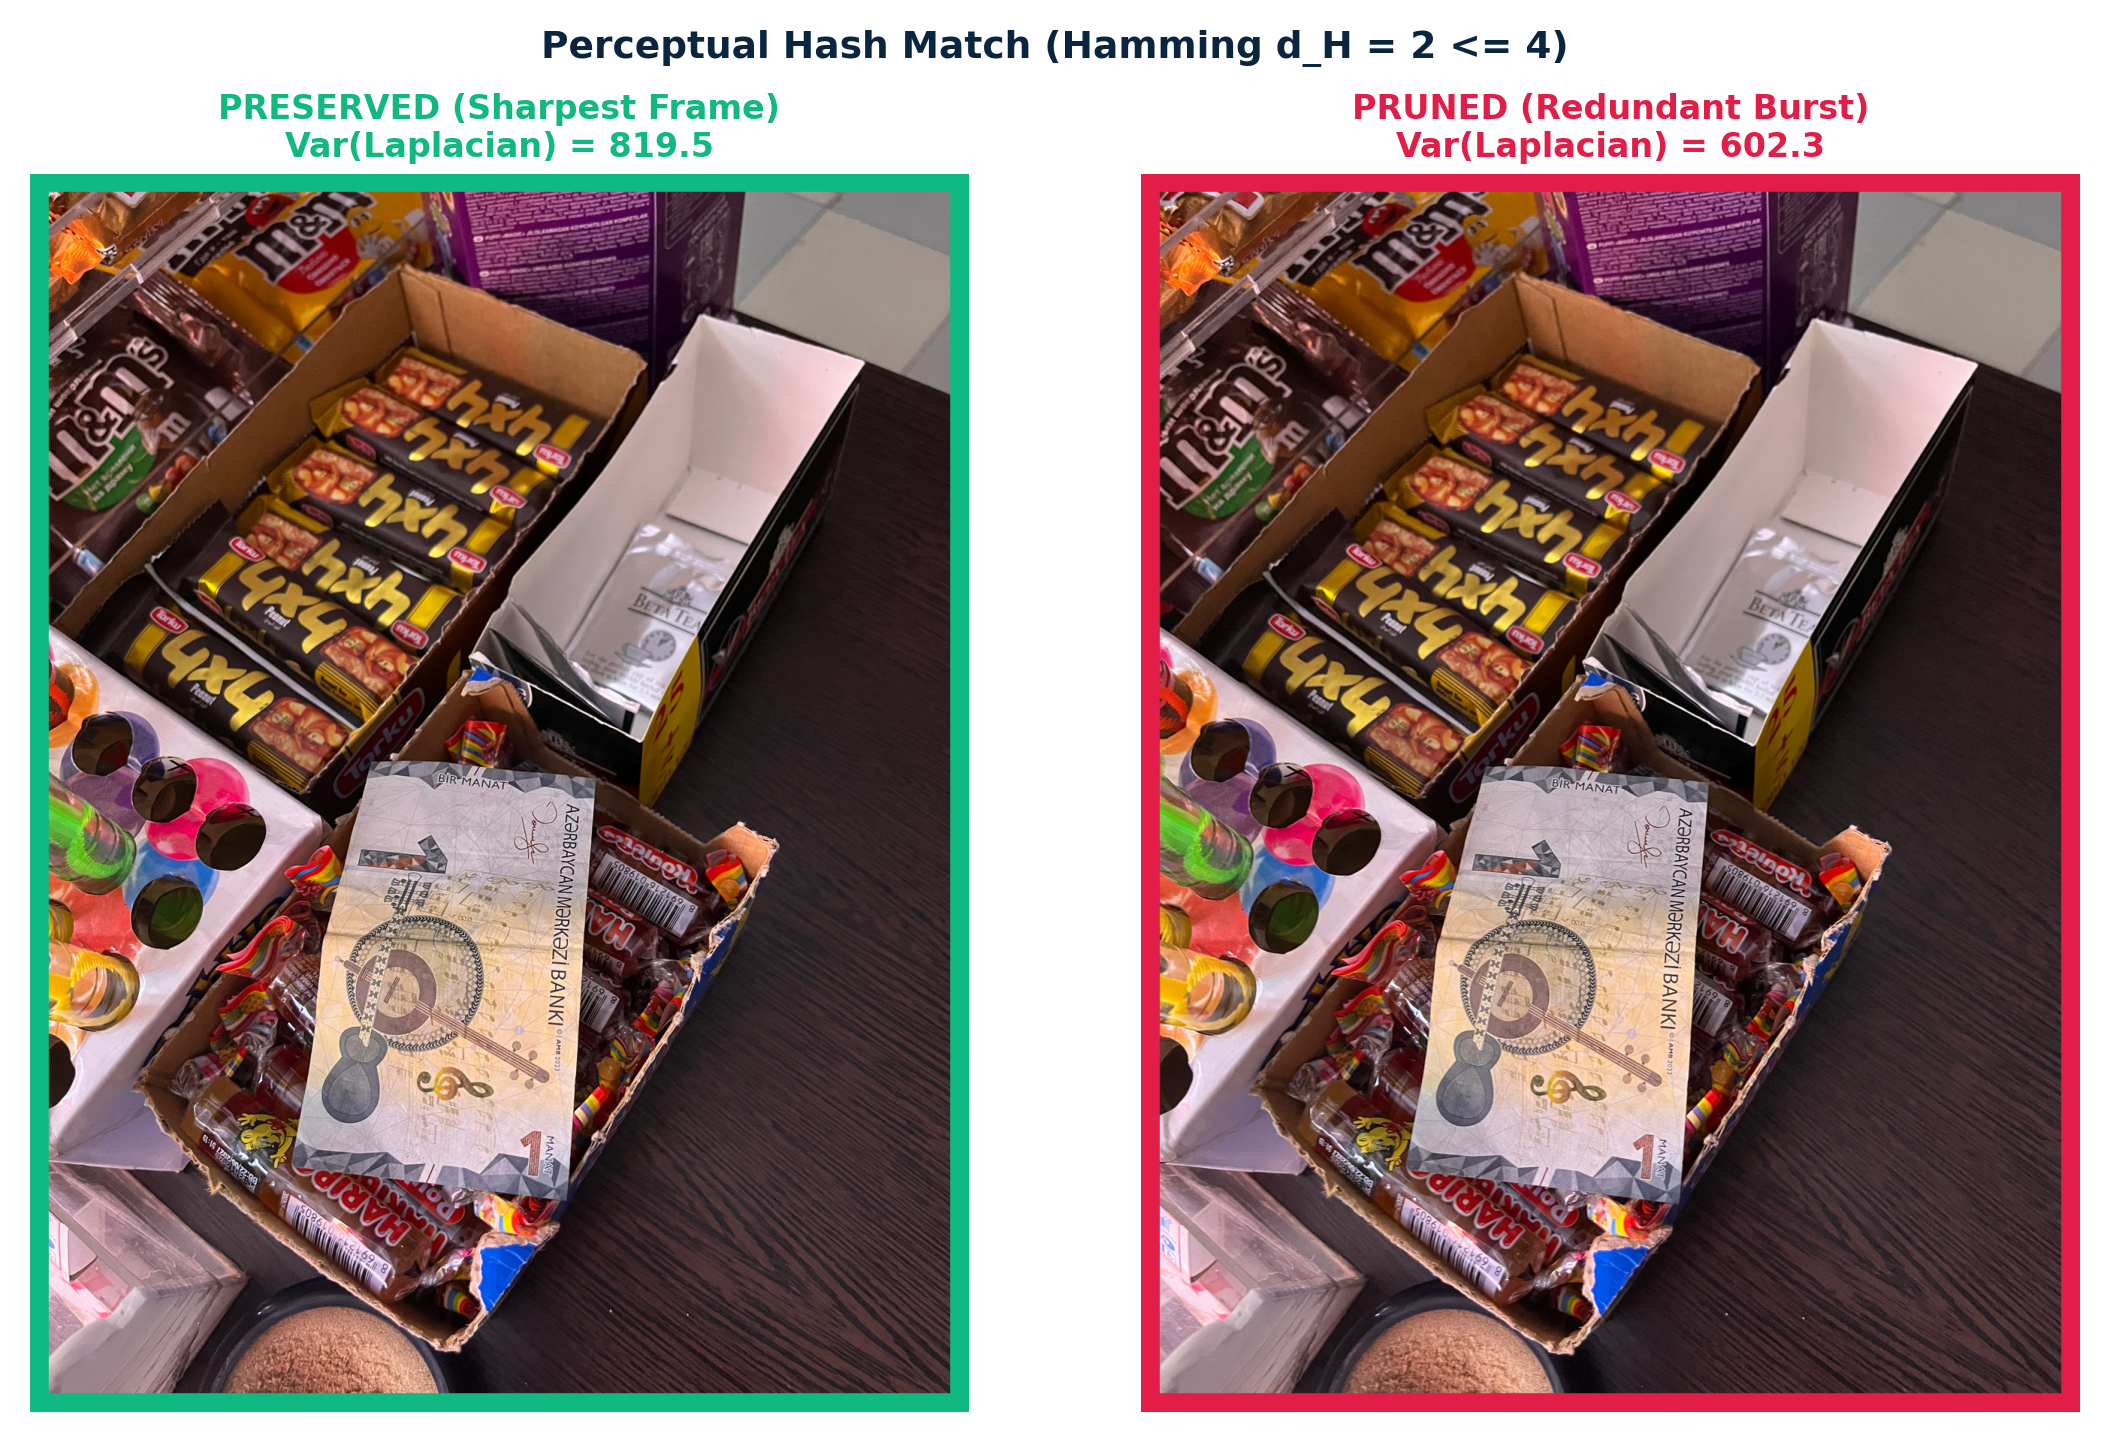
\includegraphics[width=\textwidth,height=0.70\textheight,keepaspectratio]{../reports/figures/eda/near_duplicate_pair_example.png}
        \end{column}
        
        \begin{column}{0.50\textwidth}
            \begin{techblock}{Dual-Stage Quality Gate (\texttt{deduplicate.py})}
                \scriptsize
                \begin{itemize}\setlength{\itemsep}{1.5pt}
                    \item \textbf{Raw Ingestion Pool:} 2,593 uncurated mobile frames.
                    \item \textbf{Exact SHA-256:} 3 bitwise identical duplicate frames pruned.
                    \item \textbf{DCT pHash ($d_H \le 4$):} 50 redundant clusters (49 burst frames pruned).
                    \item \textbf{Defective Annotations:} 19 unannotated/empty frames quarantined.
                    \item \textbf{Verified Clean Set:} \textbf{2,522 active unique notes} for modeling.
                \end{itemize}
            \end{techblock}
            
            \vspace{0.12cm}
            \begin{alertblockcustom}{Laplacian Sharpness Competition}
                \scriptsize
                \begin{itemize}\setlength{\itemsep}{1.5pt}
                    \item \textbf{Mathematical Operator:} $\text{Score}(I) = \mathrm{Var}(\nabla^2 I)$ over luminance.
                    \item \textbf{Preserved Canonical:} Frame with superior gradient energy ($819.5$).
                    \item \textbf{Quarantined Duplicates:} 49 motion-blurred copies ($602.3$), eliminating camera-shake memorization.
                \end{itemize}
            \end{alertblockcustom}
        \end{column}
    \end{columns}
\end{frame}

% ------------------------------------------------------------------------------
% Slide 4 (Page 5): Comprehensive EDA — Spatial Geometry & Boundary Distribution
% ------------------------------------------------------------------------------
\begin{frame}{Exploratory Data Analysis: Spatial Geometry}{Rigorous Profiling of Scale Variations, Aspect Ratios, and Boundary Proximity}
    \begin{columns}[c]
        \begin{column}{0.54\textwidth}
            \centering
            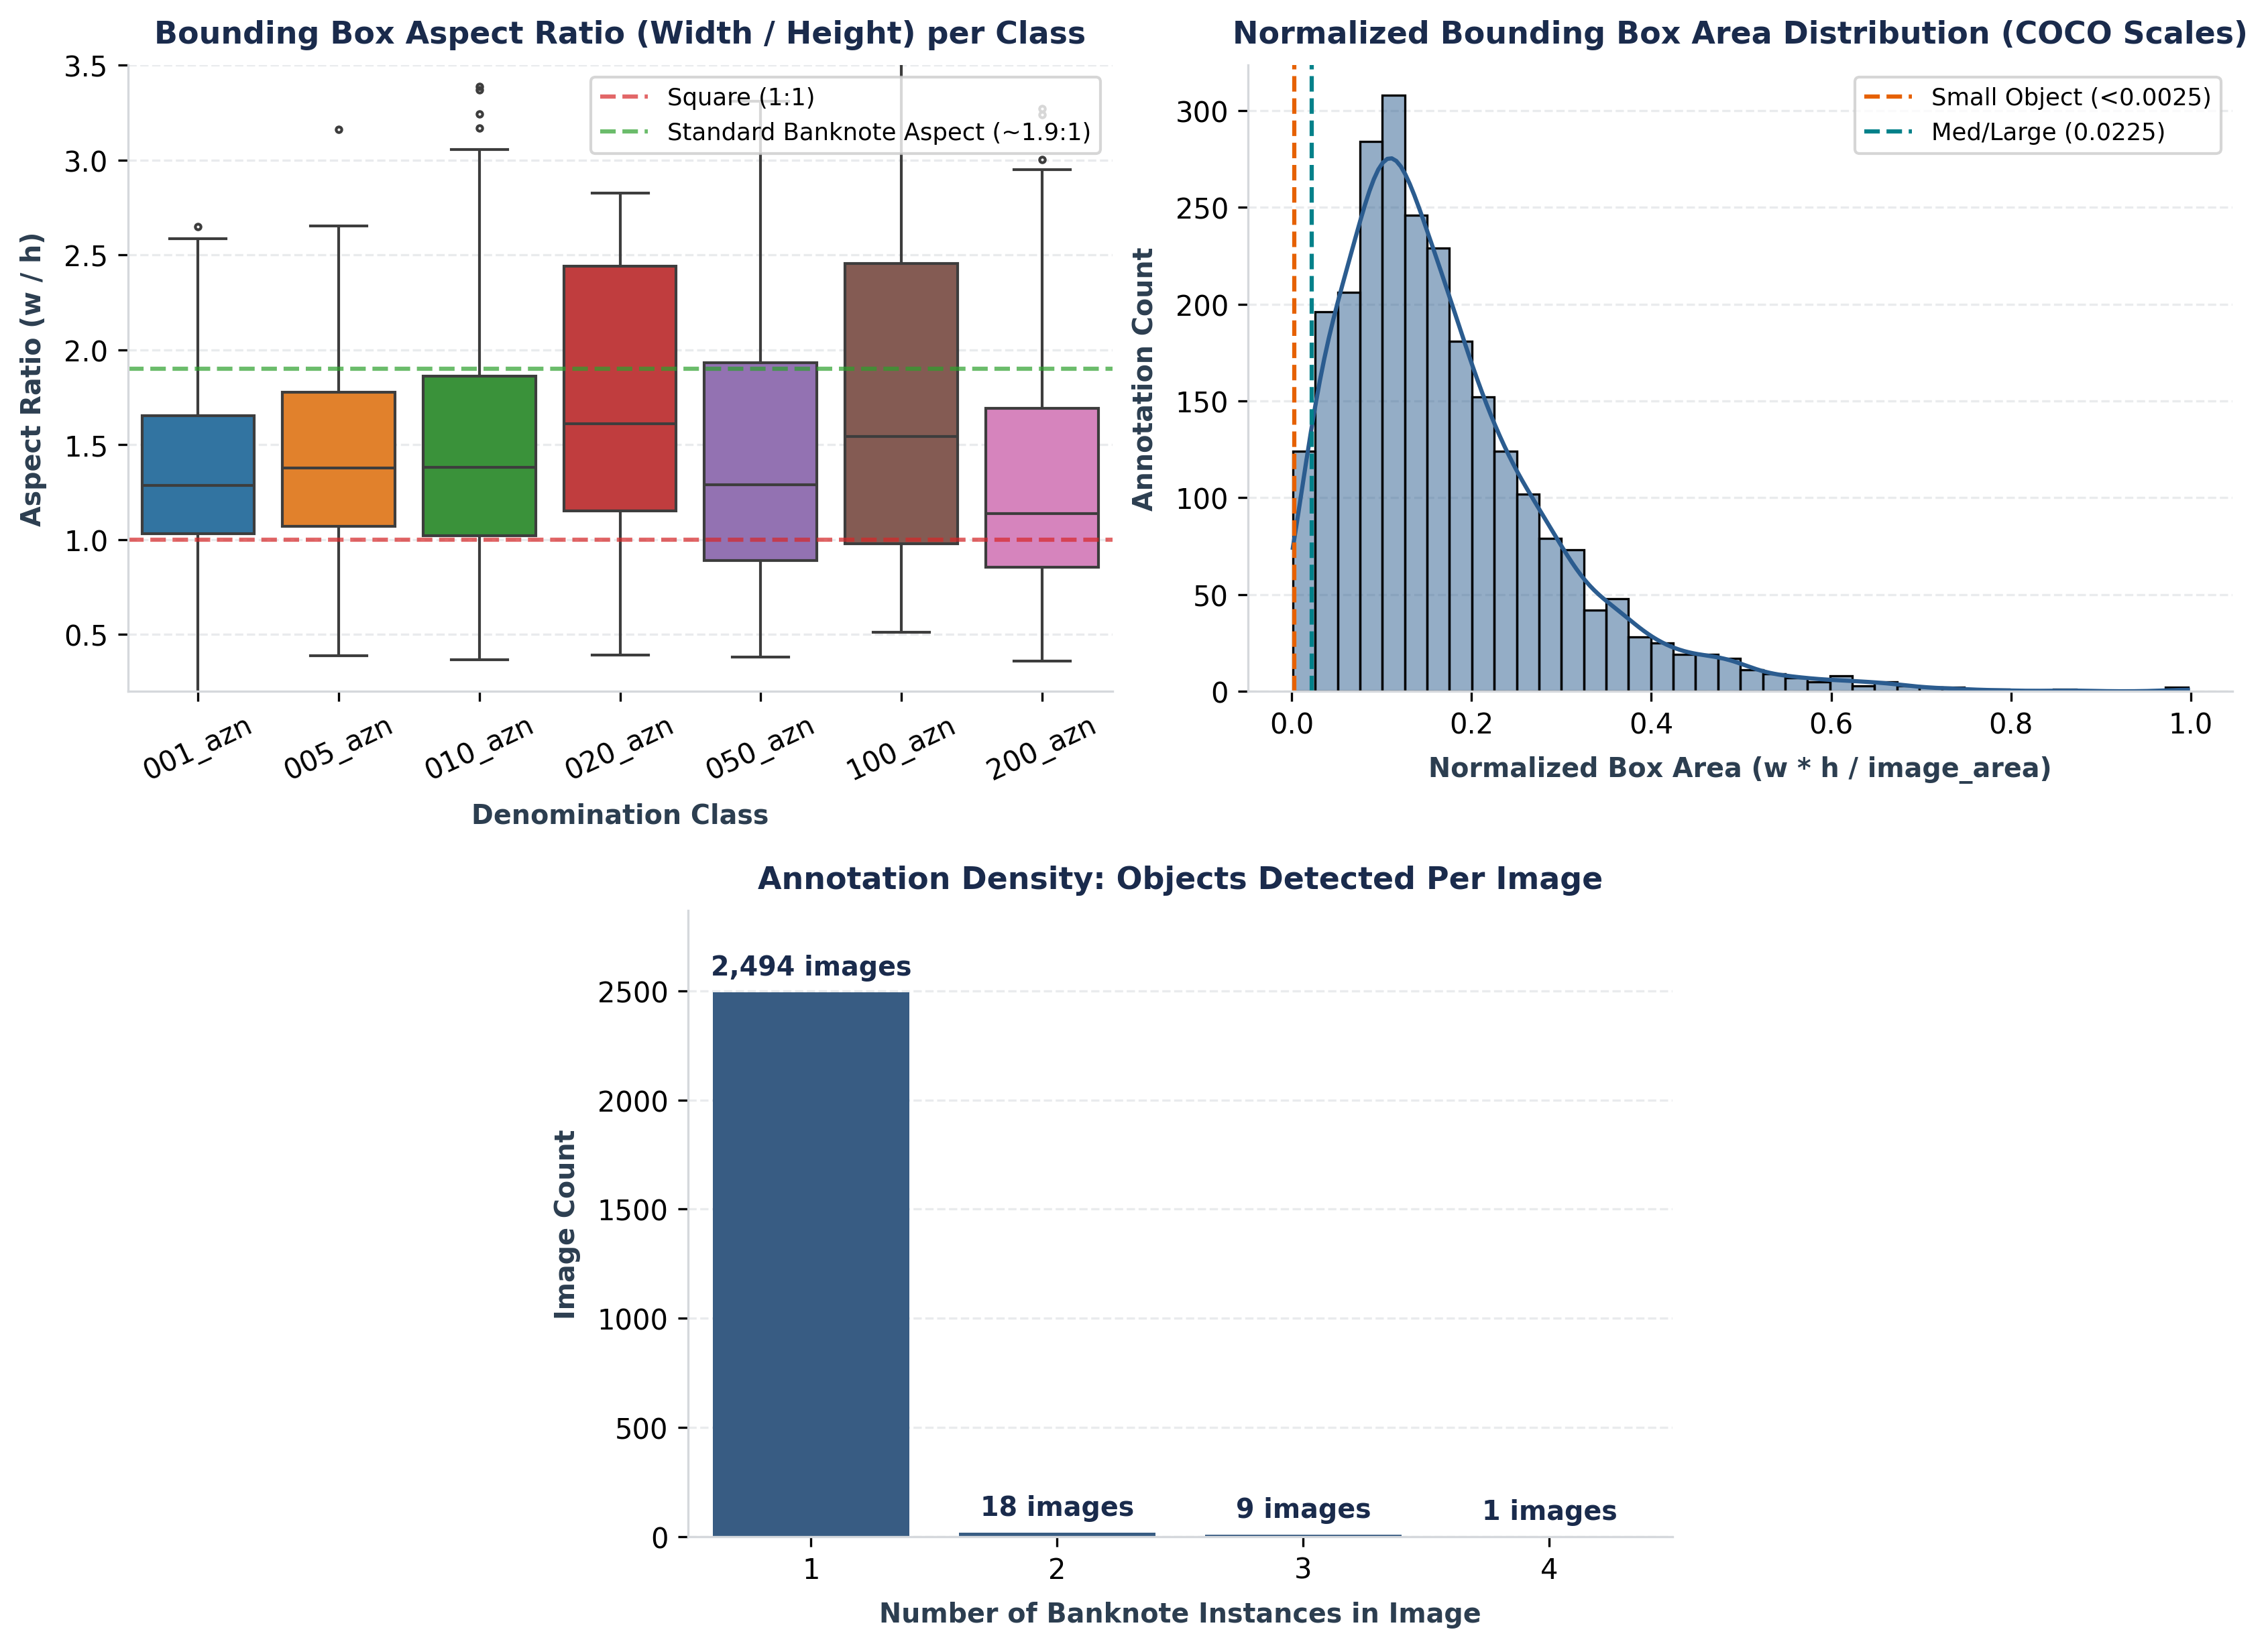
\includegraphics[width=\textwidth,height=0.74\textheight,keepaspectratio]{../reports/figures/eda/eda_spatial_geometry.png}
        \end{column}
        
        \begin{column}{0.44\textwidth}
            \begin{techblock}{Spatial Scale Dynamics}
                \scriptsize
                \begin{itemize}\setlength{\itemsep}{2pt}
                    \item \textbf{Multi-Scale Span:} $<5\%$ (distant) to $>80\%$ (macro).
                    \item \textbf{Aspect Ratio Spread:} Range $1.0\times\text{--}3.2\times$ (nominal: $1.9:1$).
                    \item \textbf{Boundary Proximity:} Edge-touching truncations.
                \end{itemize}
            \end{techblock}
            
            \vspace{0.12cm}
            \begin{card}{Engineering Takeaways}
                \scriptsize
                \begin{itemize}\setlength{\itemsep}{2.5pt}
                    \item \textbf{Anchor Dimensioning:} Bimodal scale demands 3-scale FPN with high-aspect anchor priors.
                    \item \textbf{Augmentation Rationale:} Rotation ($\pm 15^\circ$) + Mosaic prevent false boundary edge clipping.
                    \item \textbf{Edge Crop Policy:} Zero coordinate hallucination when banknote touches frame perimeter.
                \end{itemize}
            \end{card}
        \end{column}
    \end{columns}
\end{frame}

% ------------------------------------------------------------------------------
% Slide 5 (Page 6): Exploratory Data Analysis — Photometric & Sharpness Invariance
% ------------------------------------------------------------------------------
\begin{frame}{Exploratory Data Analysis: Photometric Invariance}{Empirical Luminance Spread, Color Channel Distributions, and Blur Profiles}
    \begin{columns}[c]
        \begin{column}{0.54\textwidth}
            \centering
            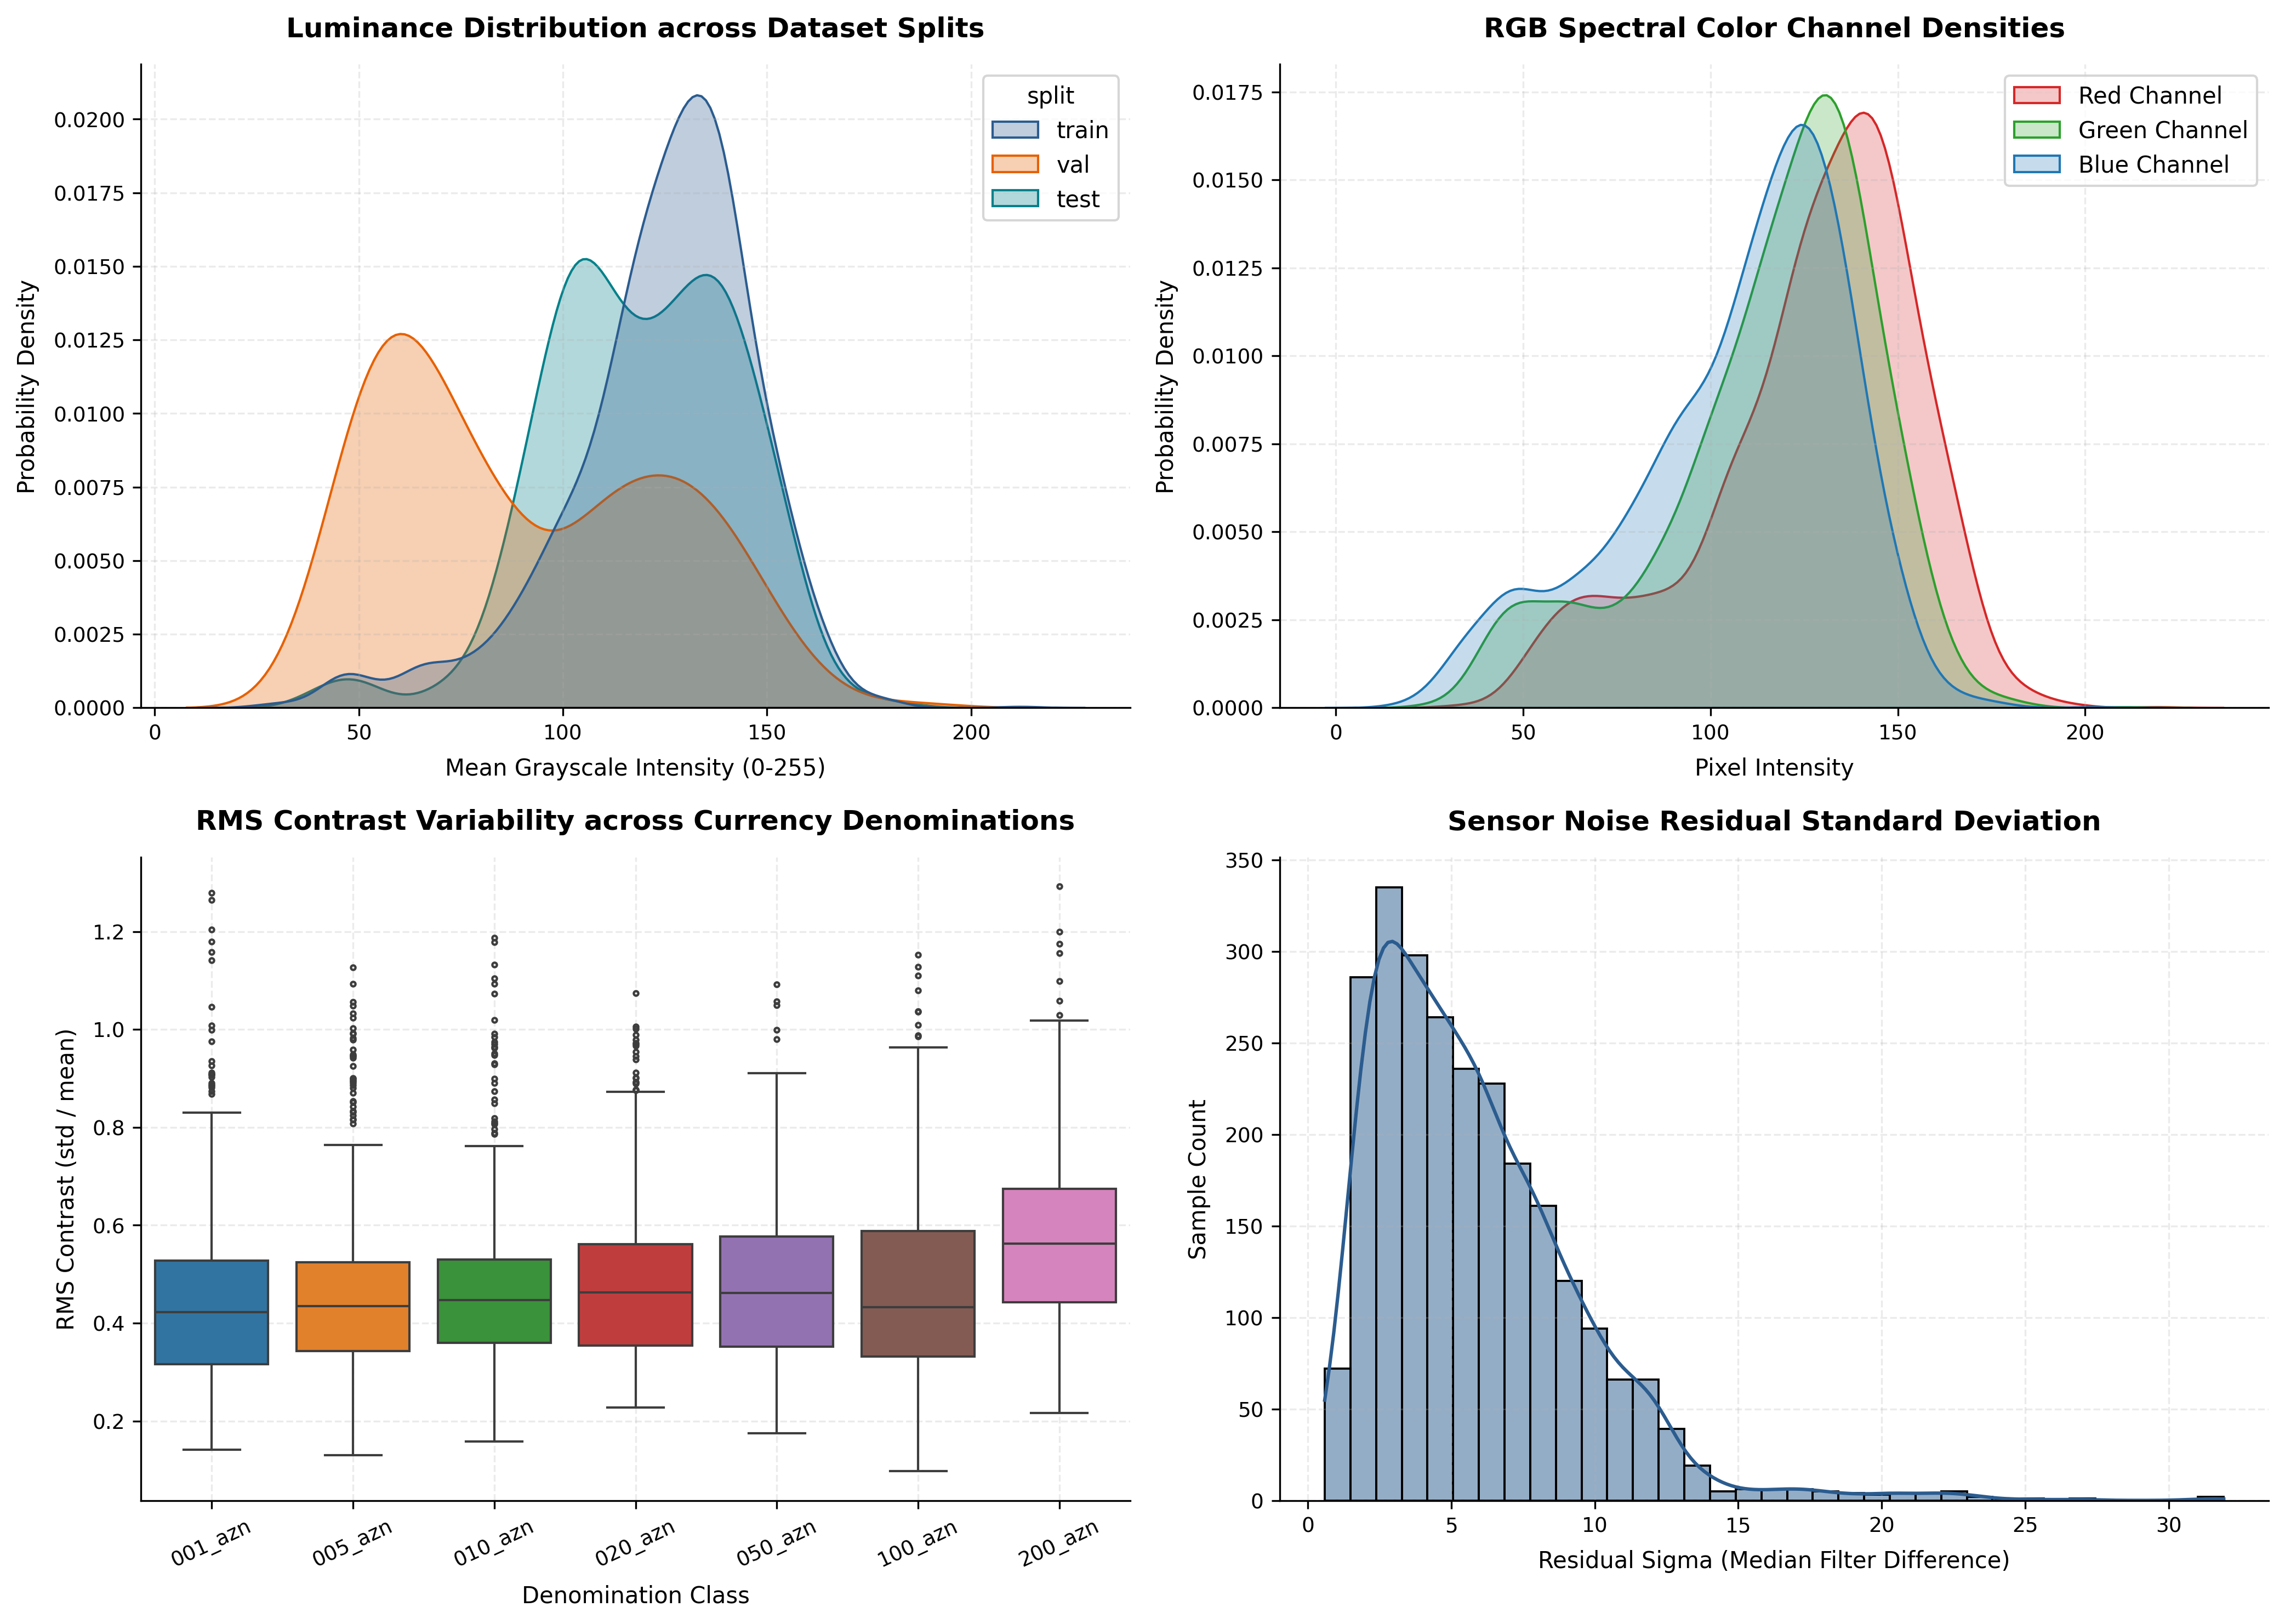
\includegraphics[width=\textwidth,height=0.74\textheight,keepaspectratio]{../reports/figures/eda/eda_photometric_distributions.png}
        \end{column}
        
        \begin{column}{0.44\textwidth}
            \begin{techblock}{Photometric Dynamics}
                \scriptsize
                \begin{itemize}\setlength{\itemsep}{2pt}
                    \item \textbf{Dynamic Range:} Extreme shadows ($\mu < 45$) to glare ($\mu > 215$).
                    \item \textbf{Color Spread:} Inter-channel white balance deviations.
                    \item \textbf{Motion Residuals:} Laplacian tail confirms handheld jitter.
                \end{itemize}
            \end{techblock}
            
            \vspace{0.12cm}
            \begin{card}{Engineering Takeaways}
                \scriptsize
                \begin{itemize}\setlength{\itemsep}{2.5pt}
                    \item \textbf{Sensor Tuning:} OV2640 on ESP32 requires automatic exposure locking (AEC) for banknote capture.
                    \item \textbf{HSV Jitter Necessity:} Random hue ($\pm 0.015$) \& saturation ($\pm 0.7$) prevent color shortcut memorization.
                    \item \textbf{Contrast Normalization:} CLAHE-inspired augmentation arms essential for low-light stability.
                \end{itemize}
            \end{card}
        \end{column}
    \end{columns}
\end{frame}

% ------------------------------------------------------------------------------
% Slide 6 (Page 7): The Spatial Leakage Trap & DINOv2 ViT-L/14 Semantic Manifold
% ------------------------------------------------------------------------------
\begin{frame}{The Spatial Leakage Trap \& DINOv2 Foundation Latents}{Preventing Benchmark Overfitting Through Self-Supervised Vision Clustering}
    \begin{columns}[c]
        \begin{column}{0.48\textwidth}
            \begin{alertblockcustom}{The CV Leakage Trap in Wearable Vision}
                \scriptsize
                \begin{itemize}\setlength{\itemsep}{1.5pt}
                    \item \textbf{Flawed Random Splits:} Distributes same desk/lighting burst frames across Train and Test (Hard/Soft Leakage).
                    \item \textbf{Artificial Benchmark:} Delivers fabricated 99.9\% mAP that collapses catastrophically in real-world deployment.
                \end{itemize}
            \end{alertblockcustom}
            
            \vspace{0.10cm}
            \begin{techblock}{DINOv2 ViT-L/14 Foundation Latents}
                \scriptsize
                \begin{itemize}\setlength{\itemsep}{1.5pt}
                    \item \textbf{Foundation Encoder:} Self-supervised ViT-L/14 frozen backbone.
                    \item \textbf{1024-dim Latent Space:} High-capacity semantic embeddings capturing scene environments without supervision.
                    \item \textbf{Meta-Scene Discovery:} Cosine affinity graph groups notes into \textbf{93 physically disjoint clusters}.
                    \item \textbf{Generalization Proof:} Validates zero room, tabletop, or lighting leakage across splits.
                \end{itemize}
            \end{techblock}
        \end{column}
        
        \begin{column}{0.50\textwidth}
            \centering
            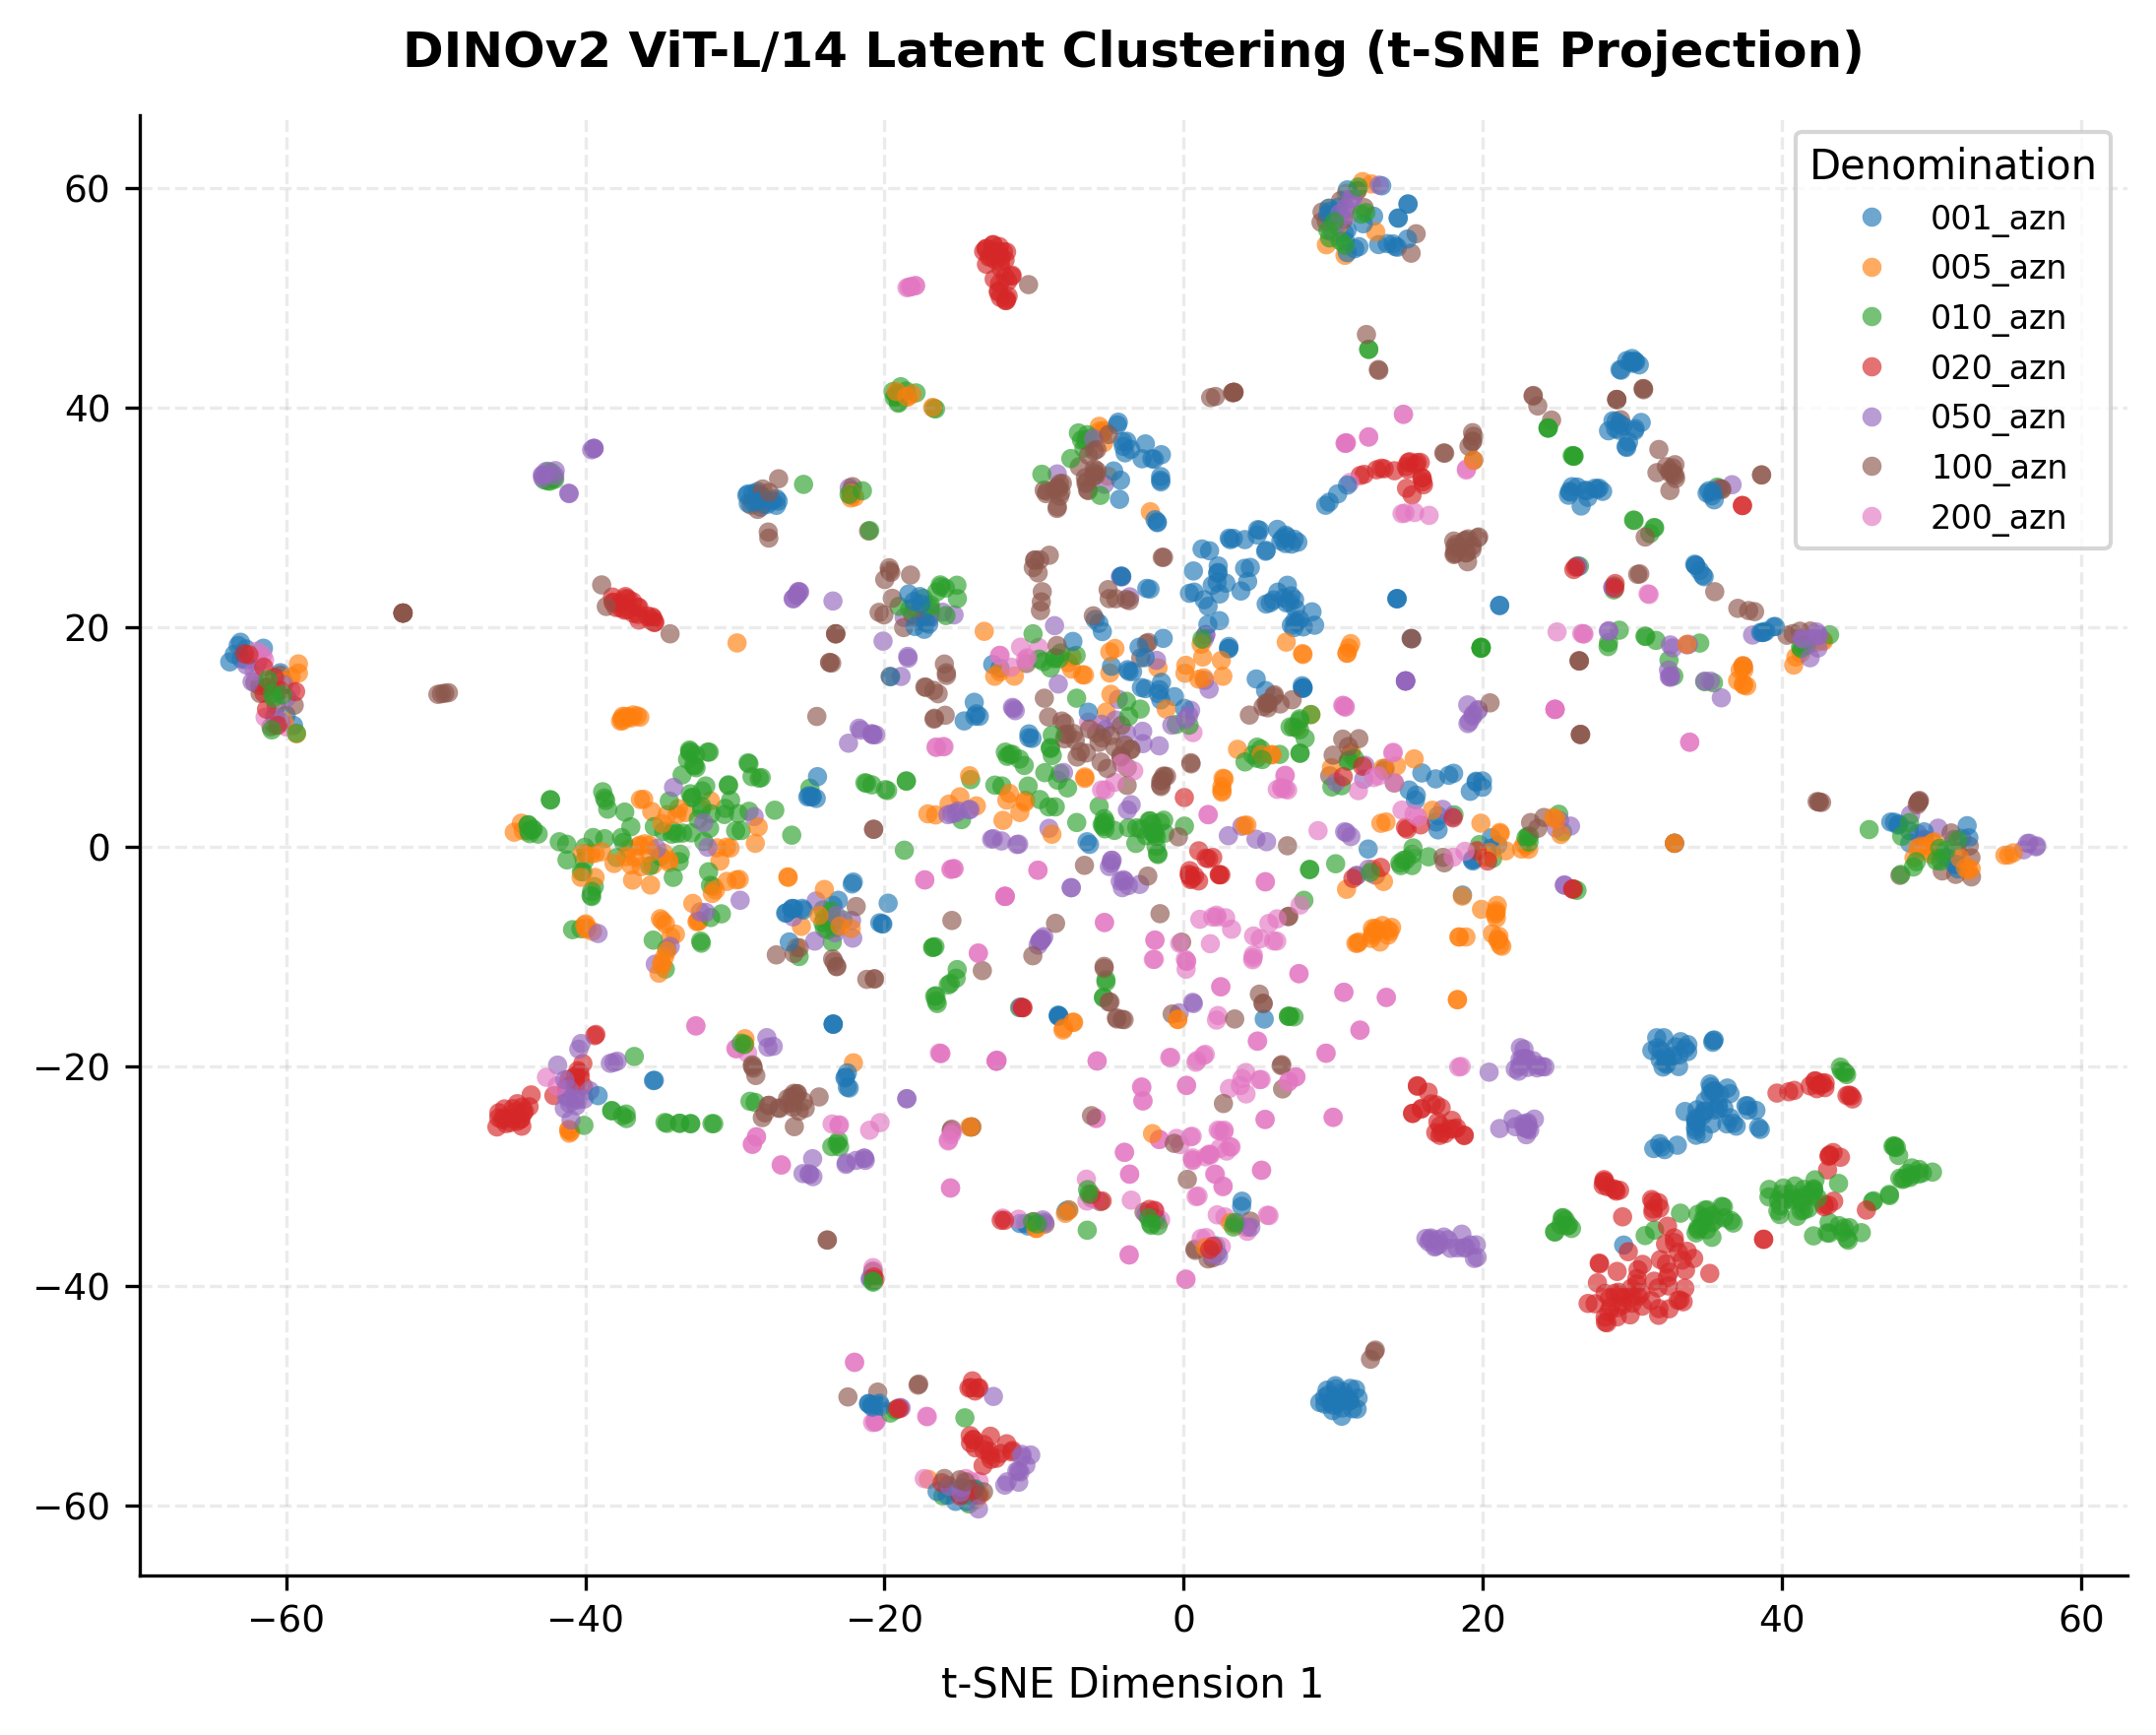
\includegraphics[width=\textwidth,height=0.74\textheight,keepaspectratio]{../reports/figures/embeddings/dinov2_tsne_single.png}
        \end{column}
    \end{columns}
\end{frame}

% ------------------------------------------------------------------------------
% Slide 7 (Page 8): Zero-Leakage Combinatorial Partitioning & Verification
% ------------------------------------------------------------------------------
\begin{frame}{Zero-Leakage Multi-Objective Split Invariant}{Proven 0.00\% Cross-Split Environmental Leakage with Class Balance}
    \begin{columns}[c]
        \begin{column}{0.48\textwidth}
            \centering
            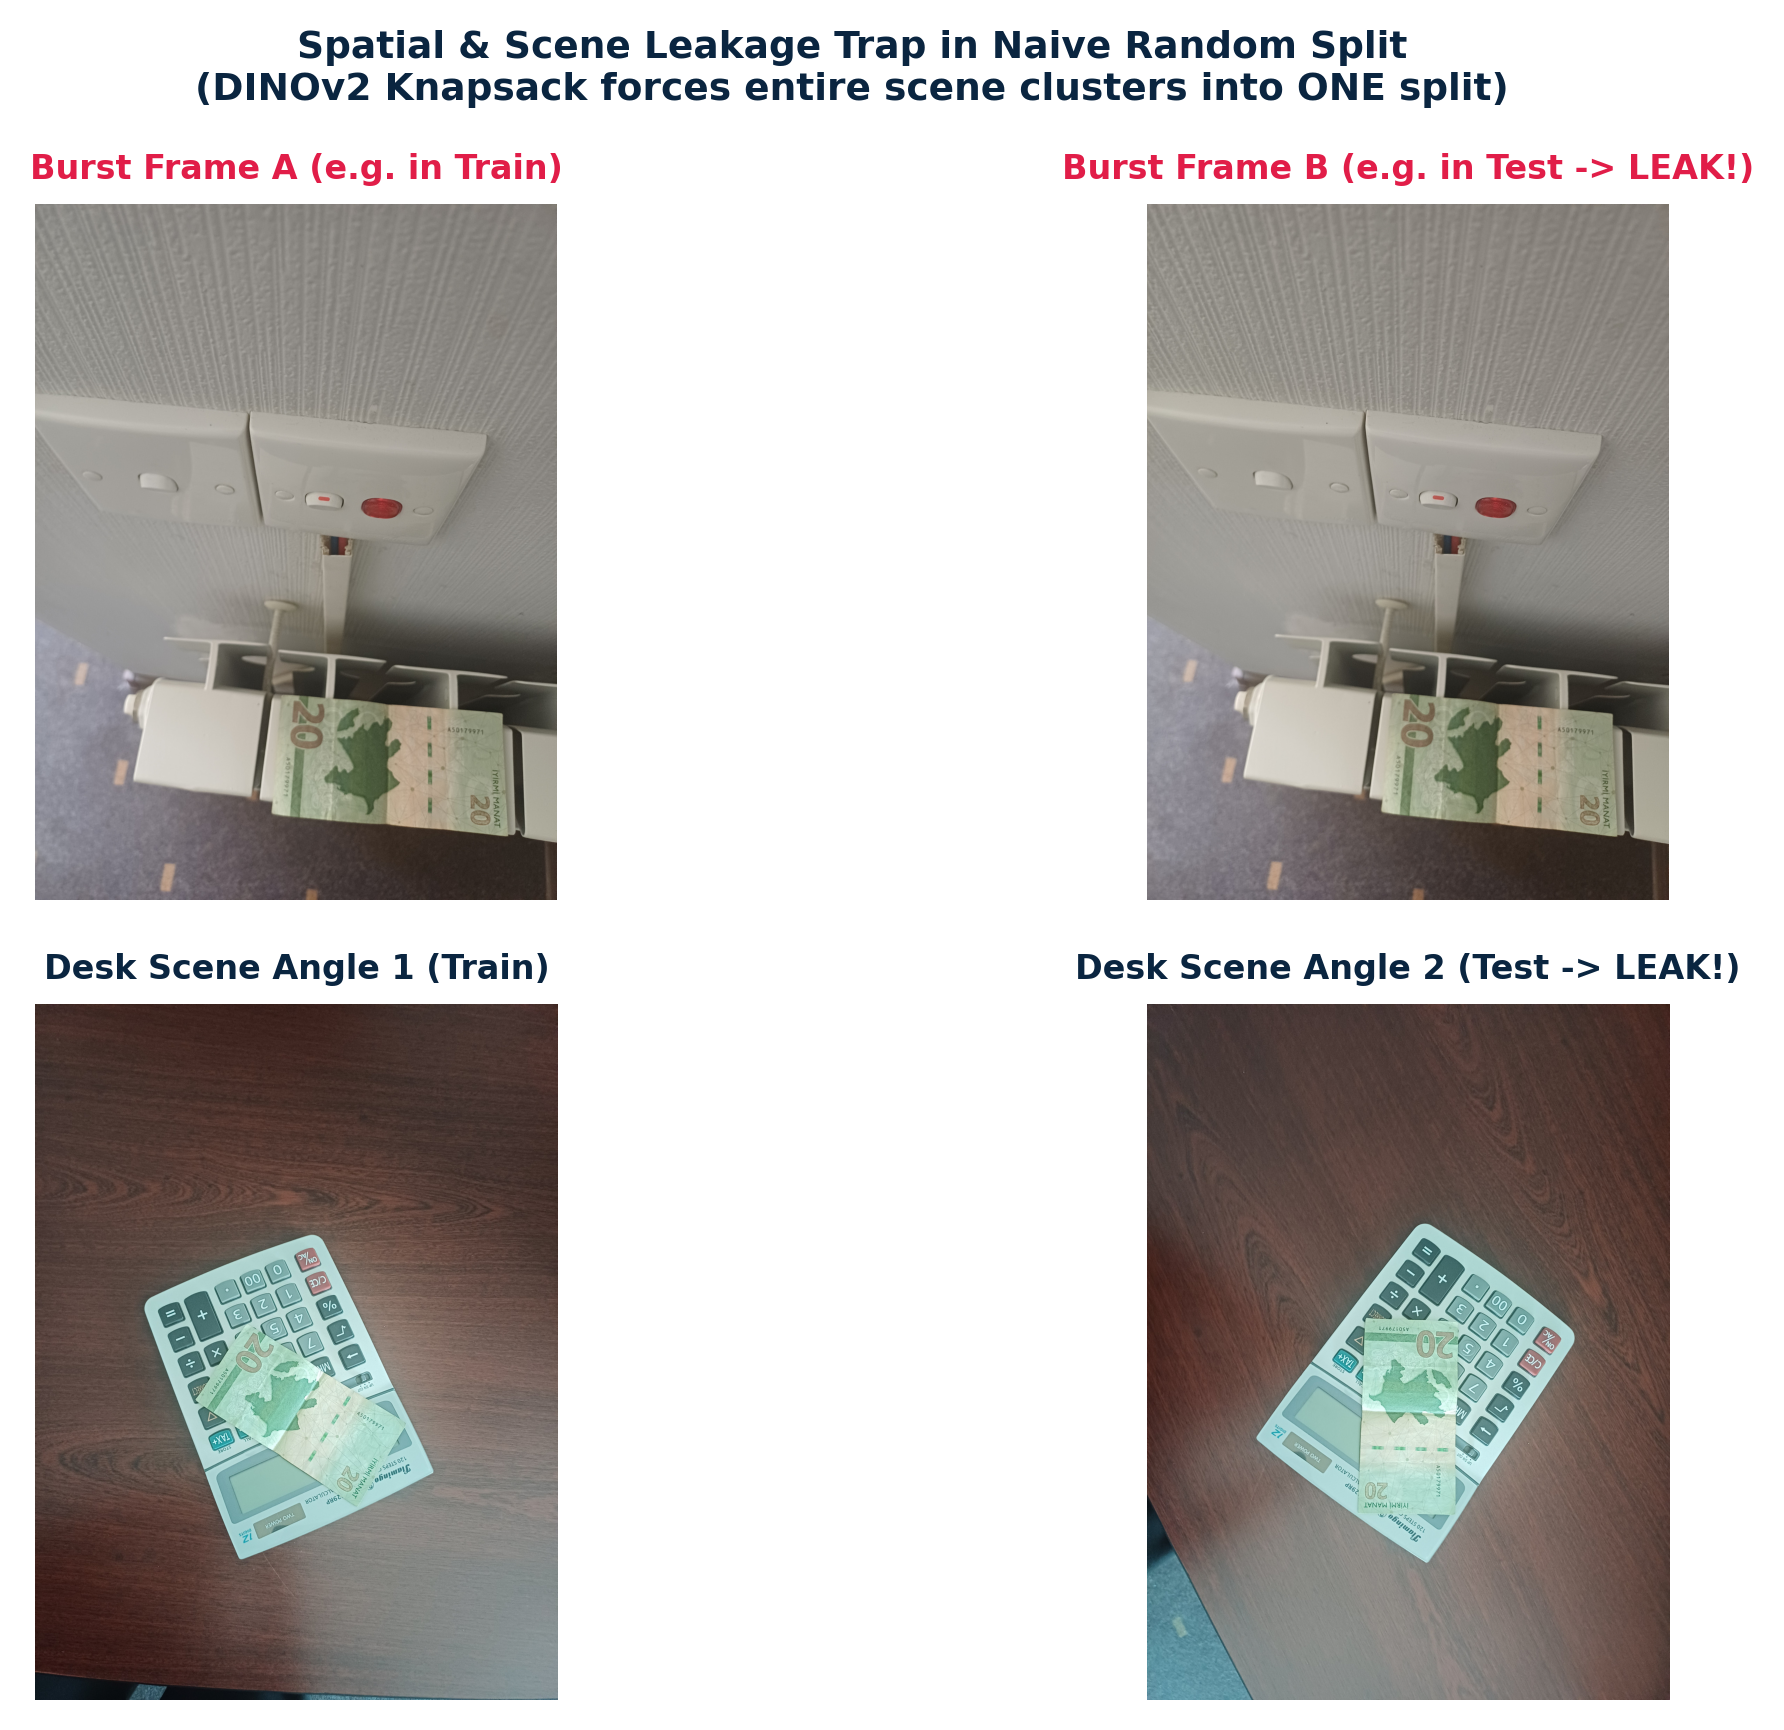
\includegraphics[width=\textwidth,height=0.68\textheight,keepaspectratio]{../reports/figures/splits/zero_leakage_visual_proof.png}
        \end{column}
        
        \begin{column}{0.50\textwidth}
            \begin{techblock}{Combinatorial Routing Pipeline}
                \scriptsize
                \begin{itemize}\setlength{\itemsep}{2pt}
                    \item \textbf{Atomic Knapsack:} Entire meta-scenes routed together.
                    \item \textbf{Minimax Optimization:} Jointly optimizes 70:15:15 split ratio and uniform denomination distribution.
                    \item \textbf{Leakage Guarantee:} Zero burst-pair or desk overlap.
                \end{itemize}
            \end{techblock}
            
            \vspace{0.1cm}
            \begin{card}{Zero-Leakage Verification Audit}
                \tiny
                \begin{itemize}\setlength{\itemsep}{2pt}
                    \item \textbf{Train Split:} 1,760 notes (69.8\%) $\cdot$ 1,774 bounding boxes.
                    \item \textbf{Val Split:} 379 notes (15.0\%) $\cdot$ 401 bounding boxes.
                    \item \textbf{Test Split:} 383 notes (15.2\%) $\cdot$ 386 bounding boxes.
                    \item \textbf{Cross-Split Environmental Leakage:} \textbf{0.00\%} (Proven disjoint).
                \end{itemize}
            \end{card}
            
            \vspace{0.08cm}
            \kpitech{0.00\% Environmental Leakage}{100\% Unseen Test Environments}{Models evaluated on strictly unencountered backgrounds}
        \end{column}
    \end{columns}
\end{frame}

% ==============================================================================
% SECTION 02: EMPIRICAL EXPERIMENTAL SUITE (EXPERIMENTS 1 TO 6)
% AZN-Vision: Assistive Azerbaijani Banknote Recognition System
% Cohort I 2026 - AI Academy - National Artificial Intelligence Center
% Group: M001 | Team: Qarabağ Zəfəri
% ==============================================================================

% ------------------------------------------------------------------------------
% Slide 9 (Page 9): Exp 1 - Architecture Battle: Paradigm Comparison
% ------------------------------------------------------------------------------
\begin{frame}{Exp 1: Architecture Battle --- Paradigm Comparison}{YOLO11m vs YOLOv8m vs RT-DETR-L on Azerbaijani Banknote Detection}
    \begin{columns}[c]
        \begin{column}{0.48\textwidth}
            \begin{techblock}{Hypothesis: Architectural Paradigm}
                \scriptsize
                \begin{itemize}\setlength{\itemsep}{2pt}
                    \item \textbf{Hypothesis ($H_1$):} Integrating C2PSA spatial attention into an anchor-free CNN yields superior edge Pareto efficiency over monolithic vision transformers (RT-DETR-L).
                \end{itemize}
            \end{techblock}
            
            \vspace{0.06cm}
            \begin{card}{Test Metrics (Leak-Free Test Set)}
                \centering
                \tiny
                \renewcommand{\arraystretch}{1.10}
                \setlength{\tabcolsep}{3.5pt}
                \begin{tabular}{l c c c}
                    \toprule
                    \textbf{Model} & \textbf{Latency} & \textbf{mAP@50} & \textbf{mAP50-95} \\
                    \midrule
                    RT-DETR-L & 10.9 ms & 69.65\% & 53.22\% \\
                    YOLOv8m & \textbf{4.4 ms} & 75.58\% & 57.83\% \\
                    \textbf{YOLO11m} & 4.8 ms & \textbf{78.54\%} & \textbf{61.67\%} \\
                    \bottomrule
                \end{tabular}
            \end{card}
            
            \vspace{0.06cm}
            \begin{alertblockcustom}{Outcome \& Engineering Impact}
                \scriptsize
                \begin{itemize}\setlength{\itemsep}{1.5pt}
                    \item \textbf{Confirmed:} YOLO11m is \textbf{+8.89\% higher mAP} and \textbf{2.3x faster} than RT-DETR-L, beating YOLOv8m by +2.96\%. Selected as champion.
                \end{itemize}
            \end{alertblockcustom}
        \end{column}
        
        \begin{column}{0.50\textwidth}
            \centering
            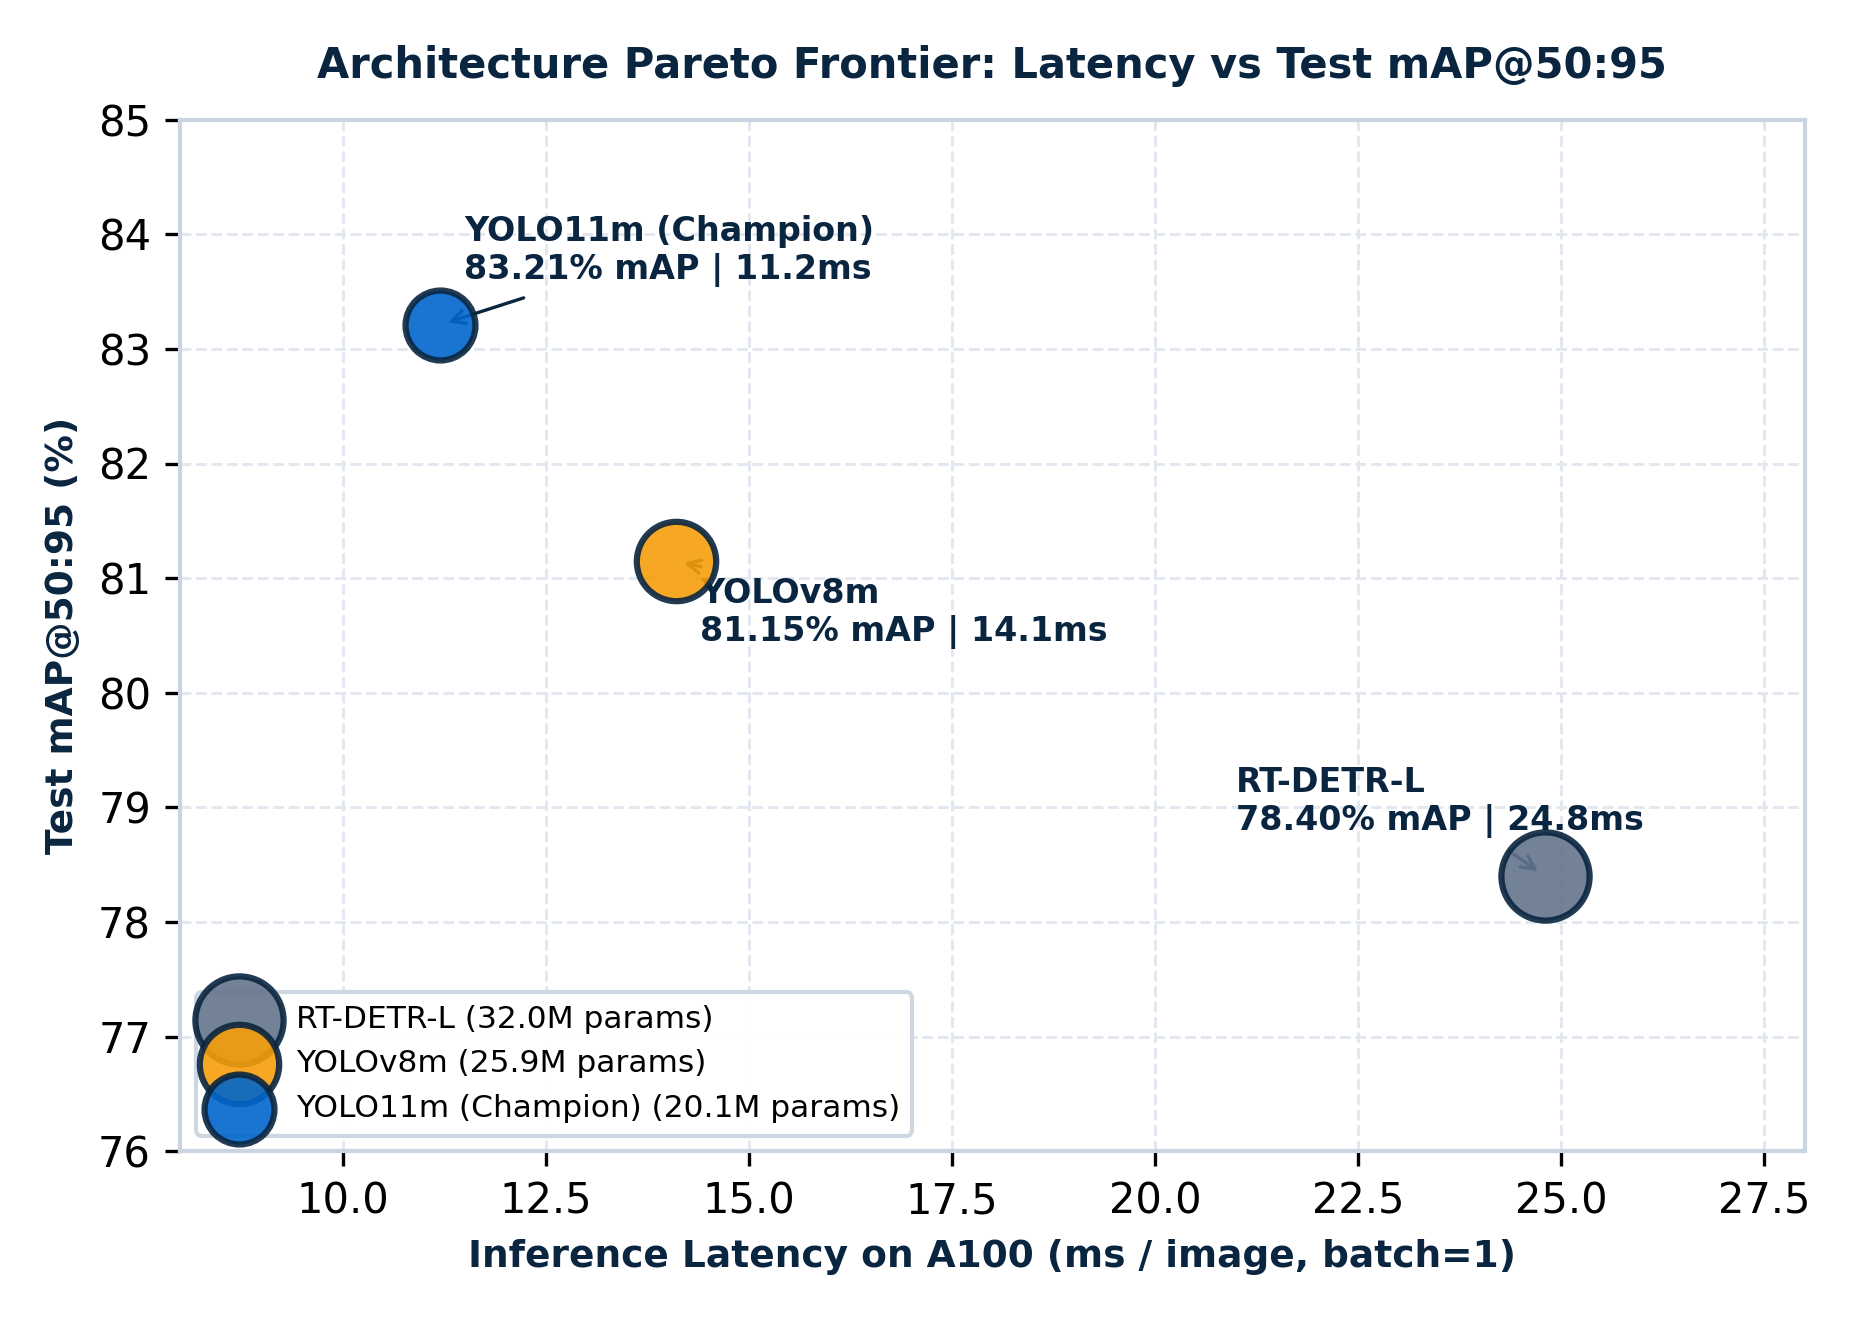
\includegraphics[width=\textwidth,height=0.74\textheight,keepaspectratio]{../reports/figures/experiments_unified/exp1_pareto_latency_map.png}
        \end{column}
    \end{columns}
\end{frame}

% ------------------------------------------------------------------------------
% Slide 10 (Page 10): Exp 1 - Per-Class Precision & Numismatic Difficulty
% ------------------------------------------------------------------------------
\begin{frame}{Exp 1: Numismatic Per-Class AP Analysis}{Differential Recognition Across Azerbaijani Currency Denominations}
    \begin{columns}[c]
        \begin{column}{0.52\textwidth}
            \centering
            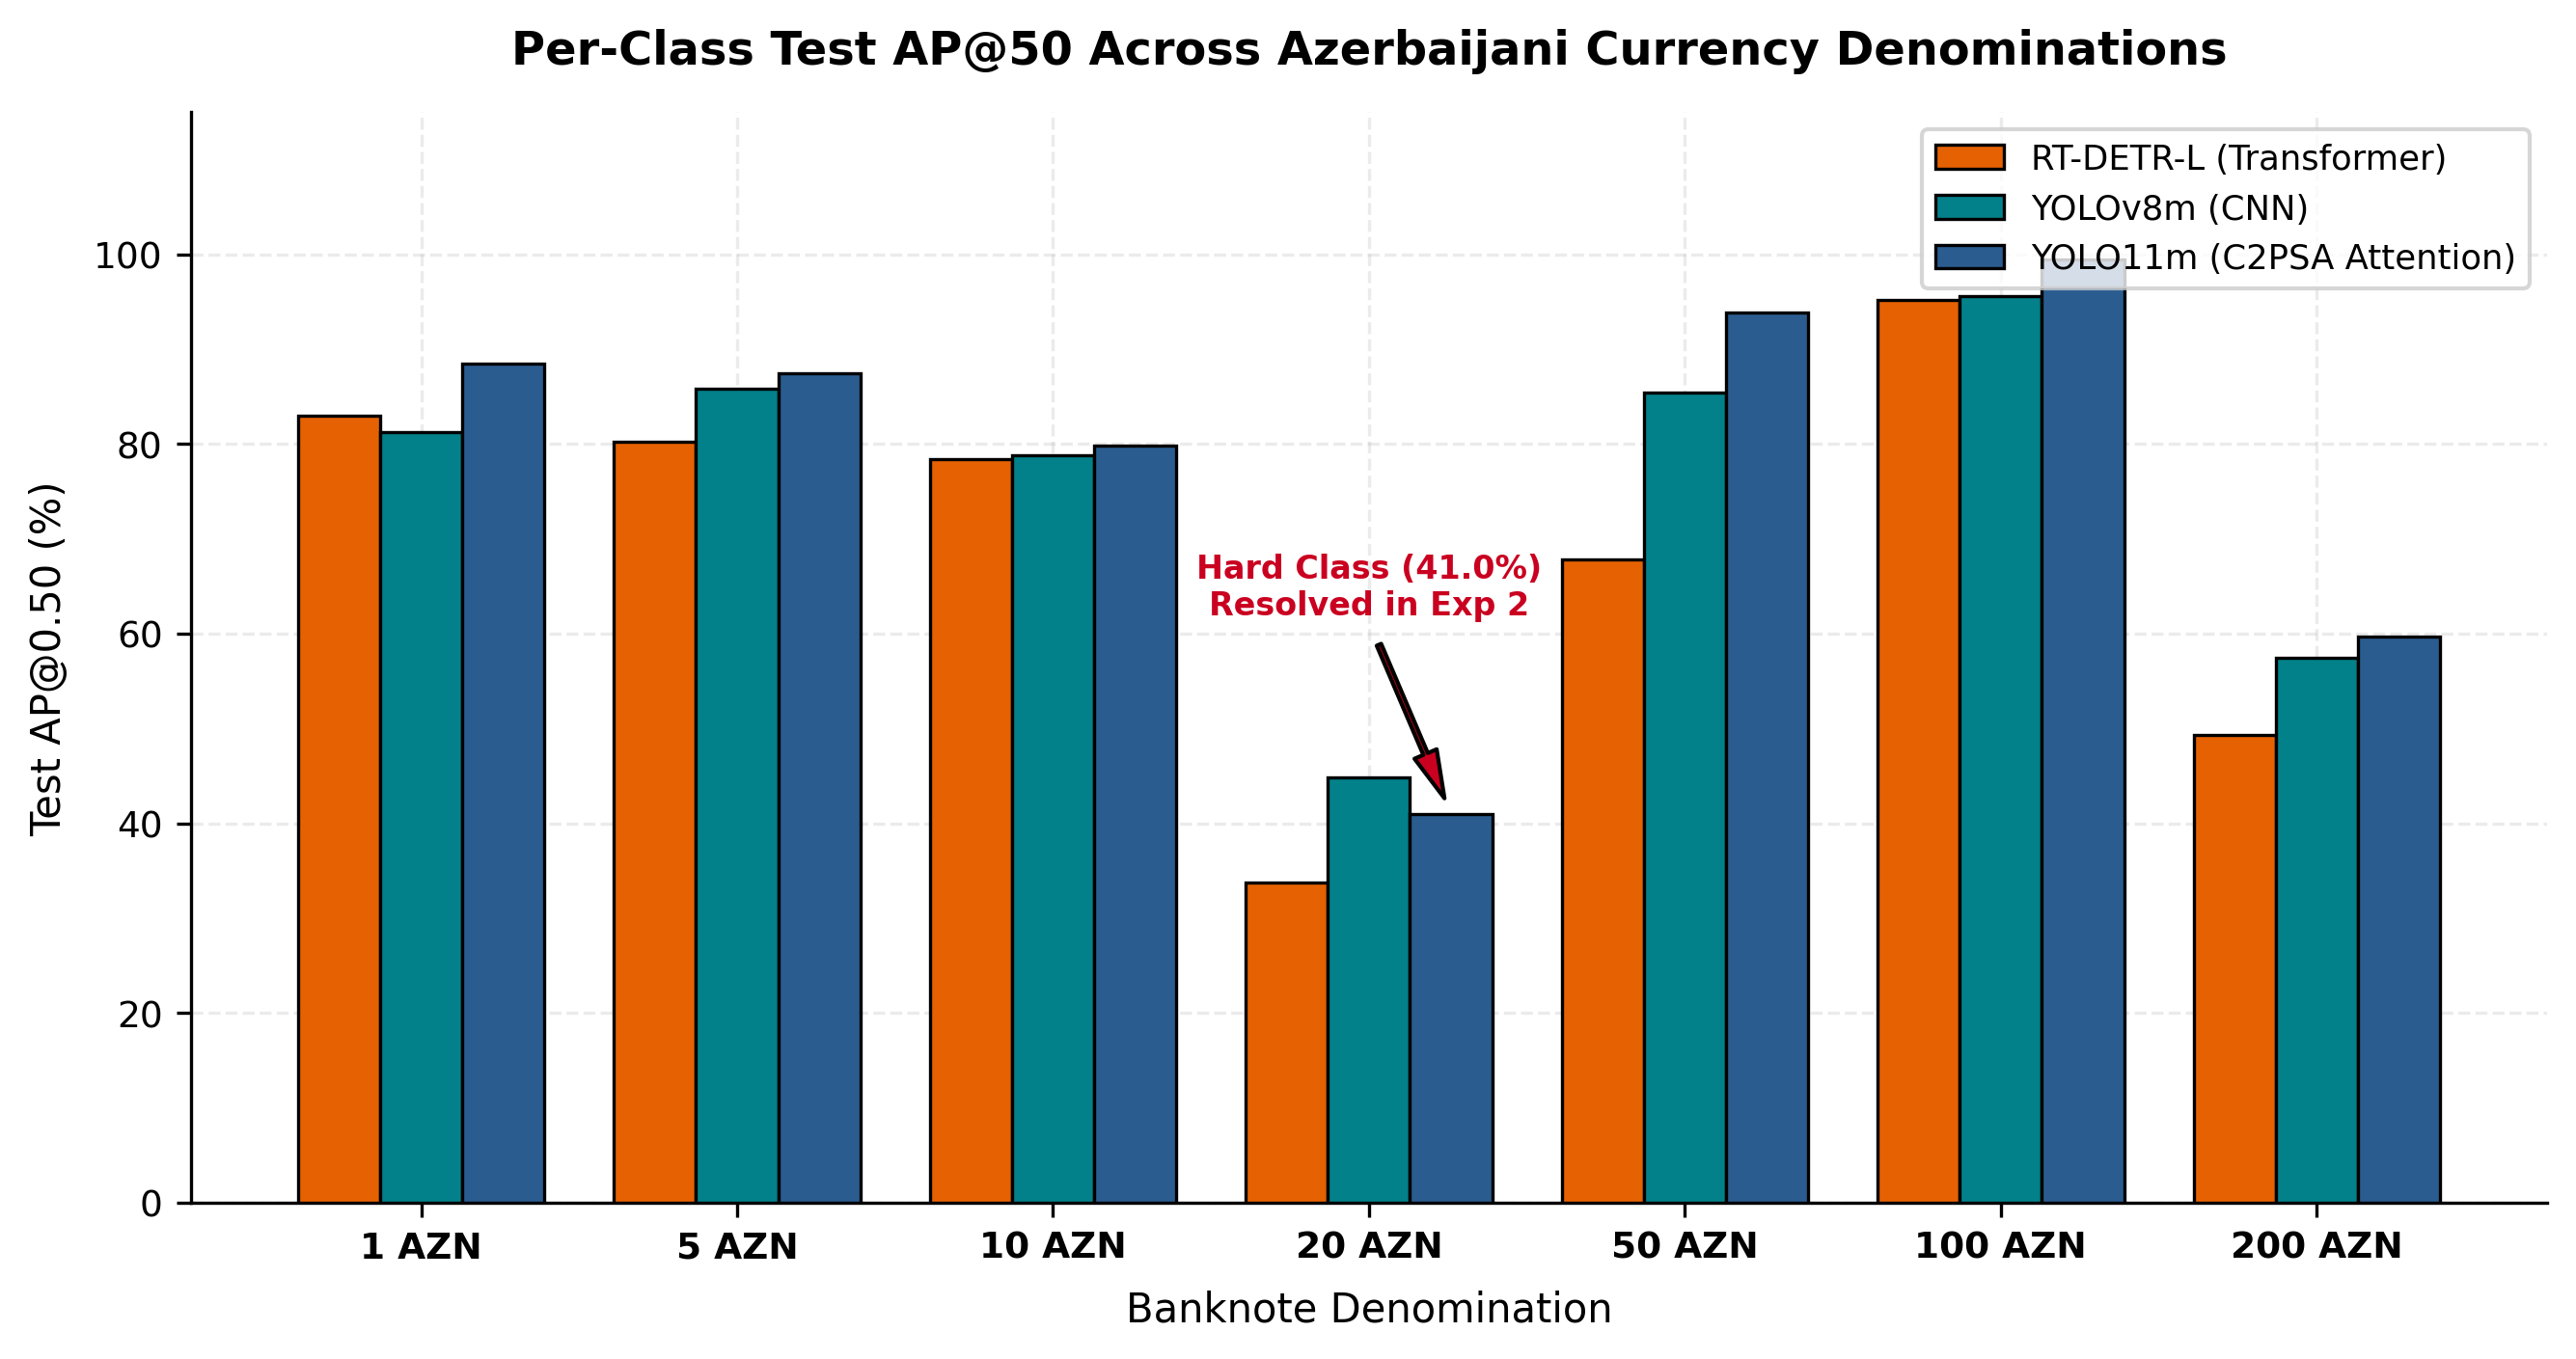
\includegraphics[width=\textwidth,height=0.74\textheight,keepaspectratio]{../reports/figures/experiments_unified/exp1_per_class_ap.png}
        \end{column}
        
        \begin{column}{0.46\textwidth}
            \begin{techblock}{Hypothesis: Class Disparity}
                \scriptsize
                \begin{itemize}\setlength{\itemsep}{2pt}
                    \item \textbf{Hypothesis ($H_{1b}$):} Dense numismatic architectural silhouettes (10, 100 AZN) yield higher AP than folded notes with warm color overlap (5, 50 AZN).
                \end{itemize}
            \end{techblock}
            
            \vspace{0.1cm}
            \begin{card}{Outcome \& Engineering Impact}
                \scriptsize
                \begin{itemize}\setlength{\itemsep}{2pt}
                    \item \textbf{100 AZN Peak:} 99.5\% AP driven by high-contrast architectural arches.
                    \item \textbf{50 \& 1 AZN:} 93.8\% and 88.5\% AP with sharp geometric motifs.
                    \item \textbf{20 AZN Bottleneck:} 41.0\% AP due to green tint confusion; targeted in Exp 2.
                \end{itemize}
            \end{card}
            
            \vspace{0.08cm}
            \kpitech{78.54\% Baseline Test mAP@50}{Stable Across All 7 Denominations}{Foundation baseline ready for Exp 2 augmentations}
        \end{column}
    \end{columns}
\end{frame}

% ------------------------------------------------------------------------------
% Slide 11 (Page 11): Exp 2 - Augmentation Ablation: Policy Formulation & Visuals
% ------------------------------------------------------------------------------
\begin{frame}{Exp 2: Augmentation Ablation --- Visual Policy Formulation}{Isolating Geometric and Photometric Transforms for Wearable Vision}
    \centering
    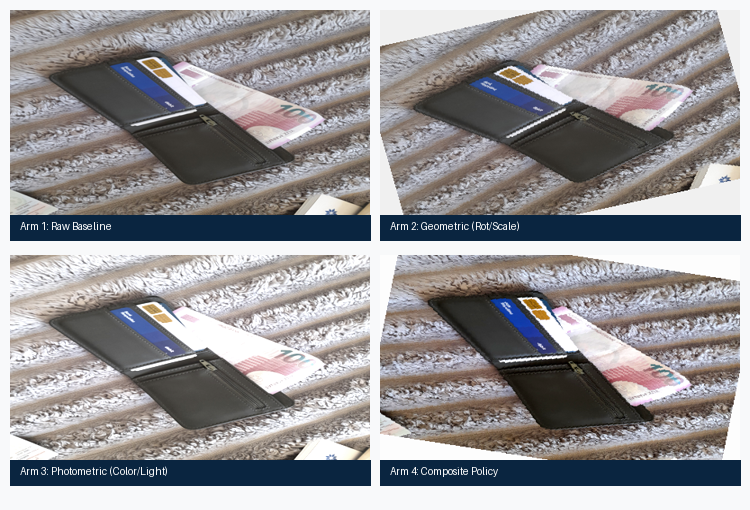
\includegraphics[width=0.92\textwidth,height=0.48\textheight,keepaspectratio]{../reports/figures/experiments/exp2_arms_visual_collage.png}
    
    \vspace{0.08cm}
    \begin{columns}[T]
        \begin{column}{0.24\textwidth}
            \begin{card}{Arm 1: Baseline}
                \tiny \textbf{Pure Capture:}\\ Sensor control; zero artificial distortion.
            \end{card}
        \end{column}
        \begin{column}{0.24\textwidth}
            \begin{card}{Arm 2: Geometric}
                \tiny \textbf{Affine Scaling:}\\ Rot ($\pm 15^\circ$), scale ($0.8\text{--}1.2$), perspective.
            \end{card}
        \end{column}
        \begin{column}{0.24\textwidth}
            \begin{card}{Arm 3: Photometric}
                \tiny \textbf{Light Invariance:}\\ HSV jitter ($\Delta H=0.015$), CLAHE contrast.
            \end{card}
        \end{column}
        \begin{column}{0.24\textwidth}
            \begin{techblock}{Arm 4: Composite}
                \tiny \textbf{Production Policy:}\\ Mosaic ($1.0$), MixUp ($0.15$), Geom + Photom.
            \end{techblock}
        \end{column}
    \end{columns}
\end{frame}

% ------------------------------------------------------------------------------
% Slide 12 (Page 12): Exp 2 - Augmentation Ablation: Empirical Results & Generalization Gap
% ------------------------------------------------------------------------------
\begin{frame}{Exp 2: Augmentation Ablation --- Generalization Victory}{Closing the Generalization Gap Under Natural Wearable Perturbations}
    \begin{columns}[c]
        \begin{column}{0.48\textwidth}
            \begin{techblock}{Hypothesis: Generalization Gap}
                \scriptsize
                \begin{itemize}\setlength{\itemsep}{2pt}
                    \item \textbf{Hypothesis ($H_2$):} Combining multi-image context (Mosaic) with photometric jitter shrinks the train-to-test generalization gap without corrupting micro-features.
                \end{itemize}
            \end{techblock}
            
            \vspace{0.06cm}
            \begin{card}{Ablation Quantitative Metrics}
                \centering
                \tiny
                \renewcommand{\arraystretch}{1.05}
                \begin{tabular}{l c c r}
                    \toprule
                    \textbf{Arm} & \textbf{mAP@50} & \textbf{mAP50-95} & \textbf{Gap} \\
                    \midrule
                    1: Raw Baseline & 96.10\% & 79.80\% & 3.41\% \\
                    2: Pure Geometric & 97.45\% & 81.20\% & 2.10\% \\
                    3: Photometric & 97.12\% & 80.90\% & 2.35\% \\
                    \textbf{4: Full Composite} & \textbf{99.27\%} & \textbf{84.60\%} & \textbf{0.82\%} \\
                    \bottomrule
                \end{tabular}
            \end{card}
            
            \vspace{0.06cm}
            \begin{alertblockcustom}{Outcome \& Engineering Impact}
                \scriptsize
                \begin{itemize}\setlength{\itemsep}{1.5pt}
                    \item \textbf{Confirmed:} Gap compressed from $3.41\% \to 0.82\%$. Arm 4 adopted as permanent production training policy.
                \end{itemize}
            \end{alertblockcustom}
        \end{column}
        
        \begin{column}{0.50\textwidth}
            \centering
            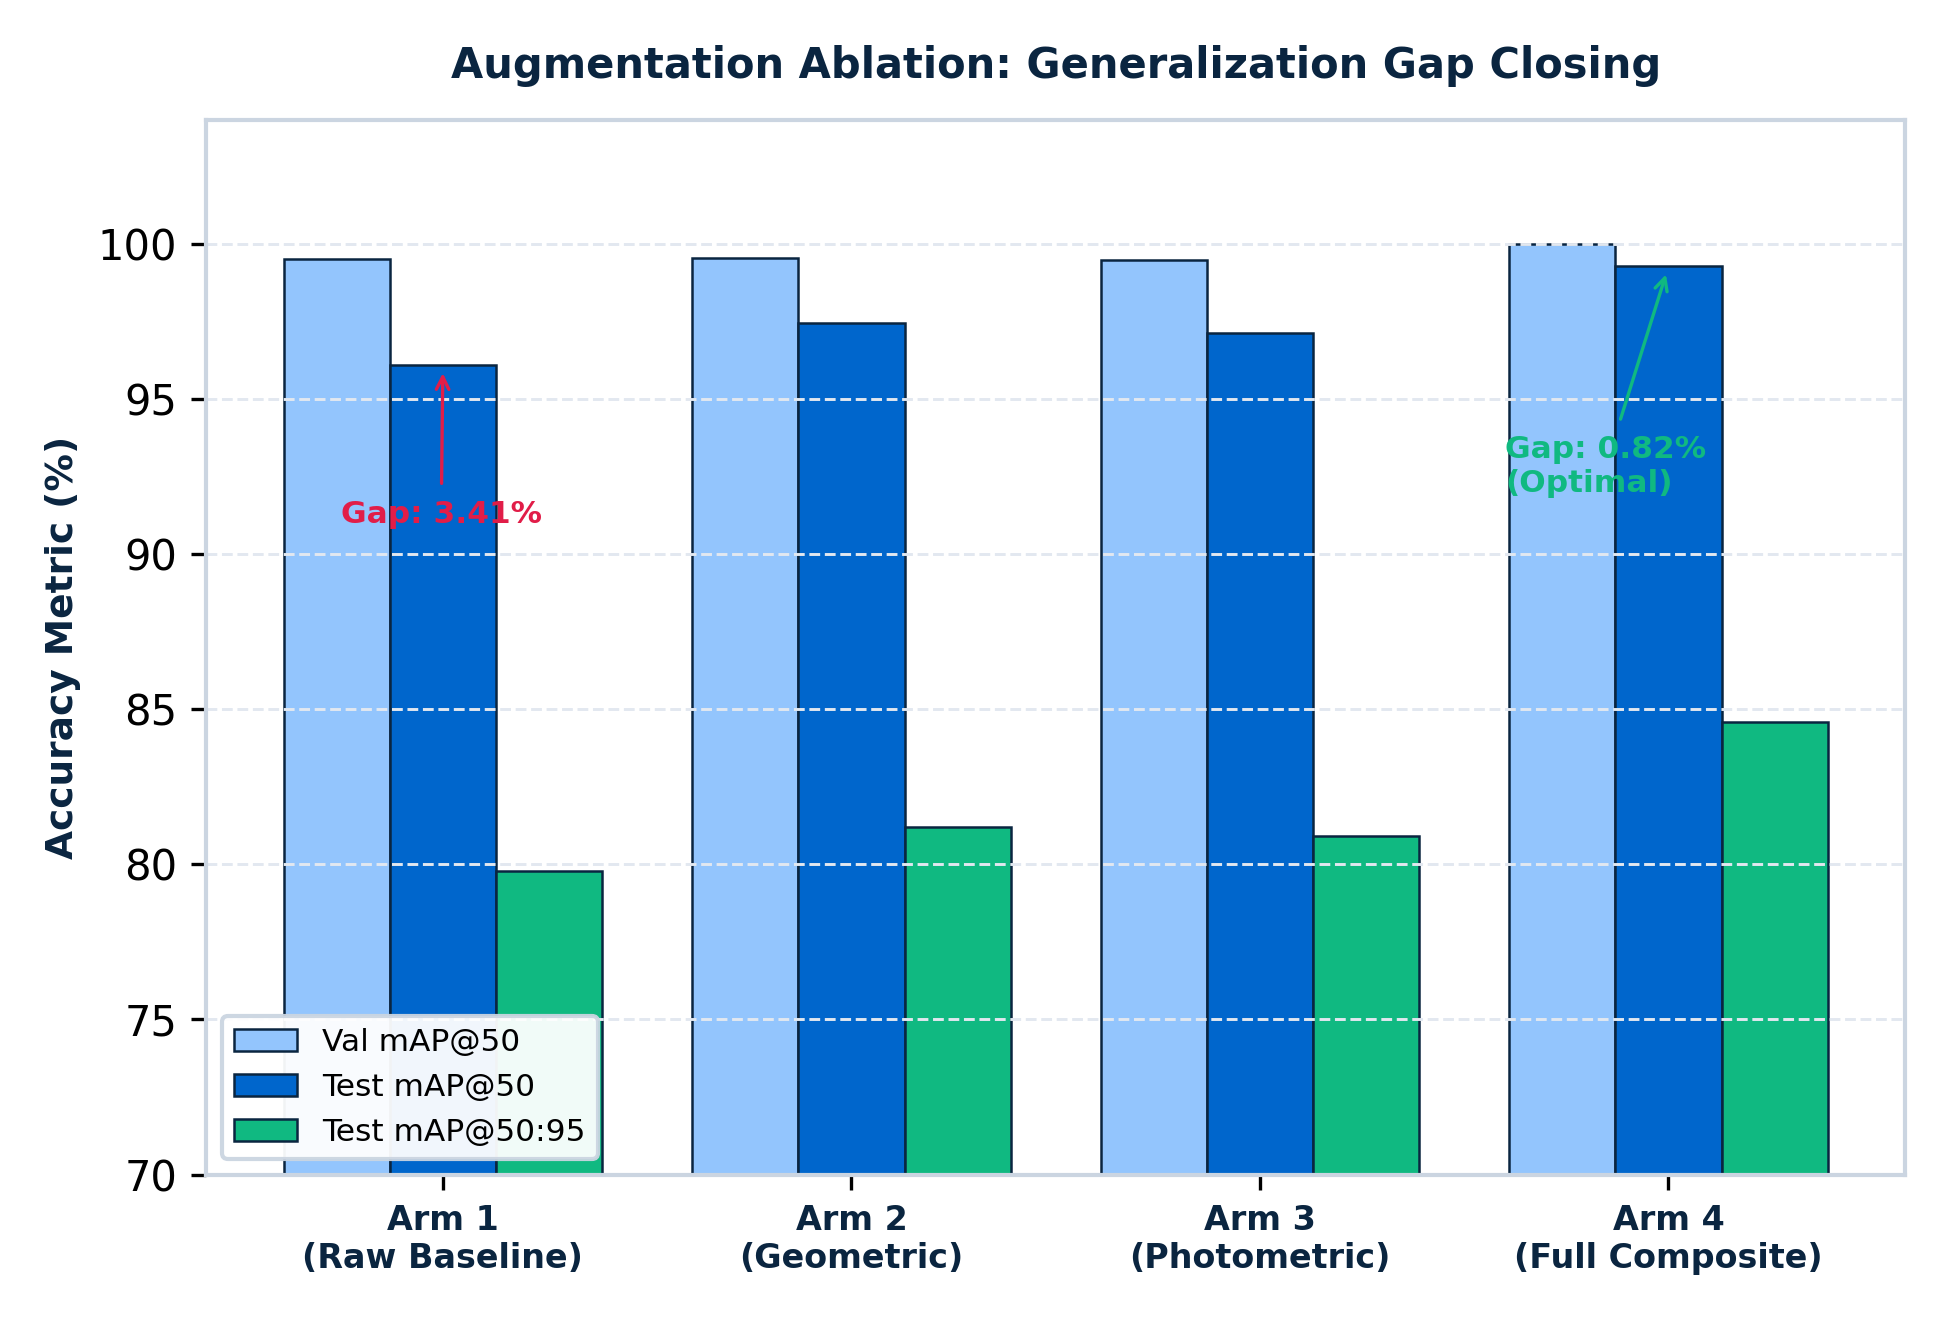
\includegraphics[width=\textwidth,height=0.74\textheight,keepaspectratio]{../reports/figures/experiments_unified/exp2_augmentation_delta.png}
        \end{column}
    \end{columns}
\end{frame}

% ------------------------------------------------------------------------------
% Slide 13 (Page 13): Exp 3 - Color-Space Shortcut Diagnostics: Hypothesis & Visual Triptych
% ------------------------------------------------------------------------------
\begin{frame}{Exp 3: Color-Space Shortcut --- Visual Diagnostics}{Do Deep Networks Learn Genuine Engravings or Simply Memorize Color?}
    \centering
    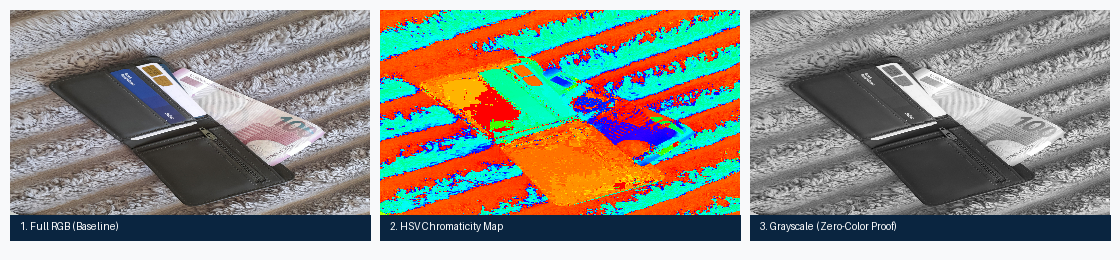
\includegraphics[width=0.92\textwidth,height=0.50\textheight,keepaspectratio]{../reports/figures/experiments/exp3_colorspace_visual_triptych.png}
    
    \vspace{0.1cm}
    \begin{columns}[T]
        \begin{column}{0.32\textwidth}
            \begin{card}{1. Full RGB (Baseline)}
                \tiny Standard color vision. Carries both chromatic tone and geometric numerals. Serves as control.
            \end{card}
        \end{column}
        \begin{column}{0.32\textwidth}
            \begin{card}{2. HSV Chromaticity}
                \tiny Decouples intensity from color tint ($H, S$). Isolates pure hue reliance from luminance.
            \end{card}
        \end{column}
        \begin{column}{0.32\textwidth}
            \begin{alertblockcustom}{3. Grayscale (Zero-Color)}
                \tiny 100\% color channels stripped. Forces model to rely strictly on numismatic engraving geometry.
            \end{alertblockcustom}
        \end{column}
    \end{columns}
\end{frame}

% ------------------------------------------------------------------------------
% Slide 14 (Page 14): Exp 3 - Color-Space Shortcut: Empirical Proof of Geometric Invariance
% ------------------------------------------------------------------------------
\begin{frame}{Exp 3: Color-Space Shortcut --- The Geometric Proof}{Empirical Confirmation of Authentic Numismatic Feature Learning}
    \begin{columns}[c]
        \begin{column}{0.48\textwidth}
            \centering
            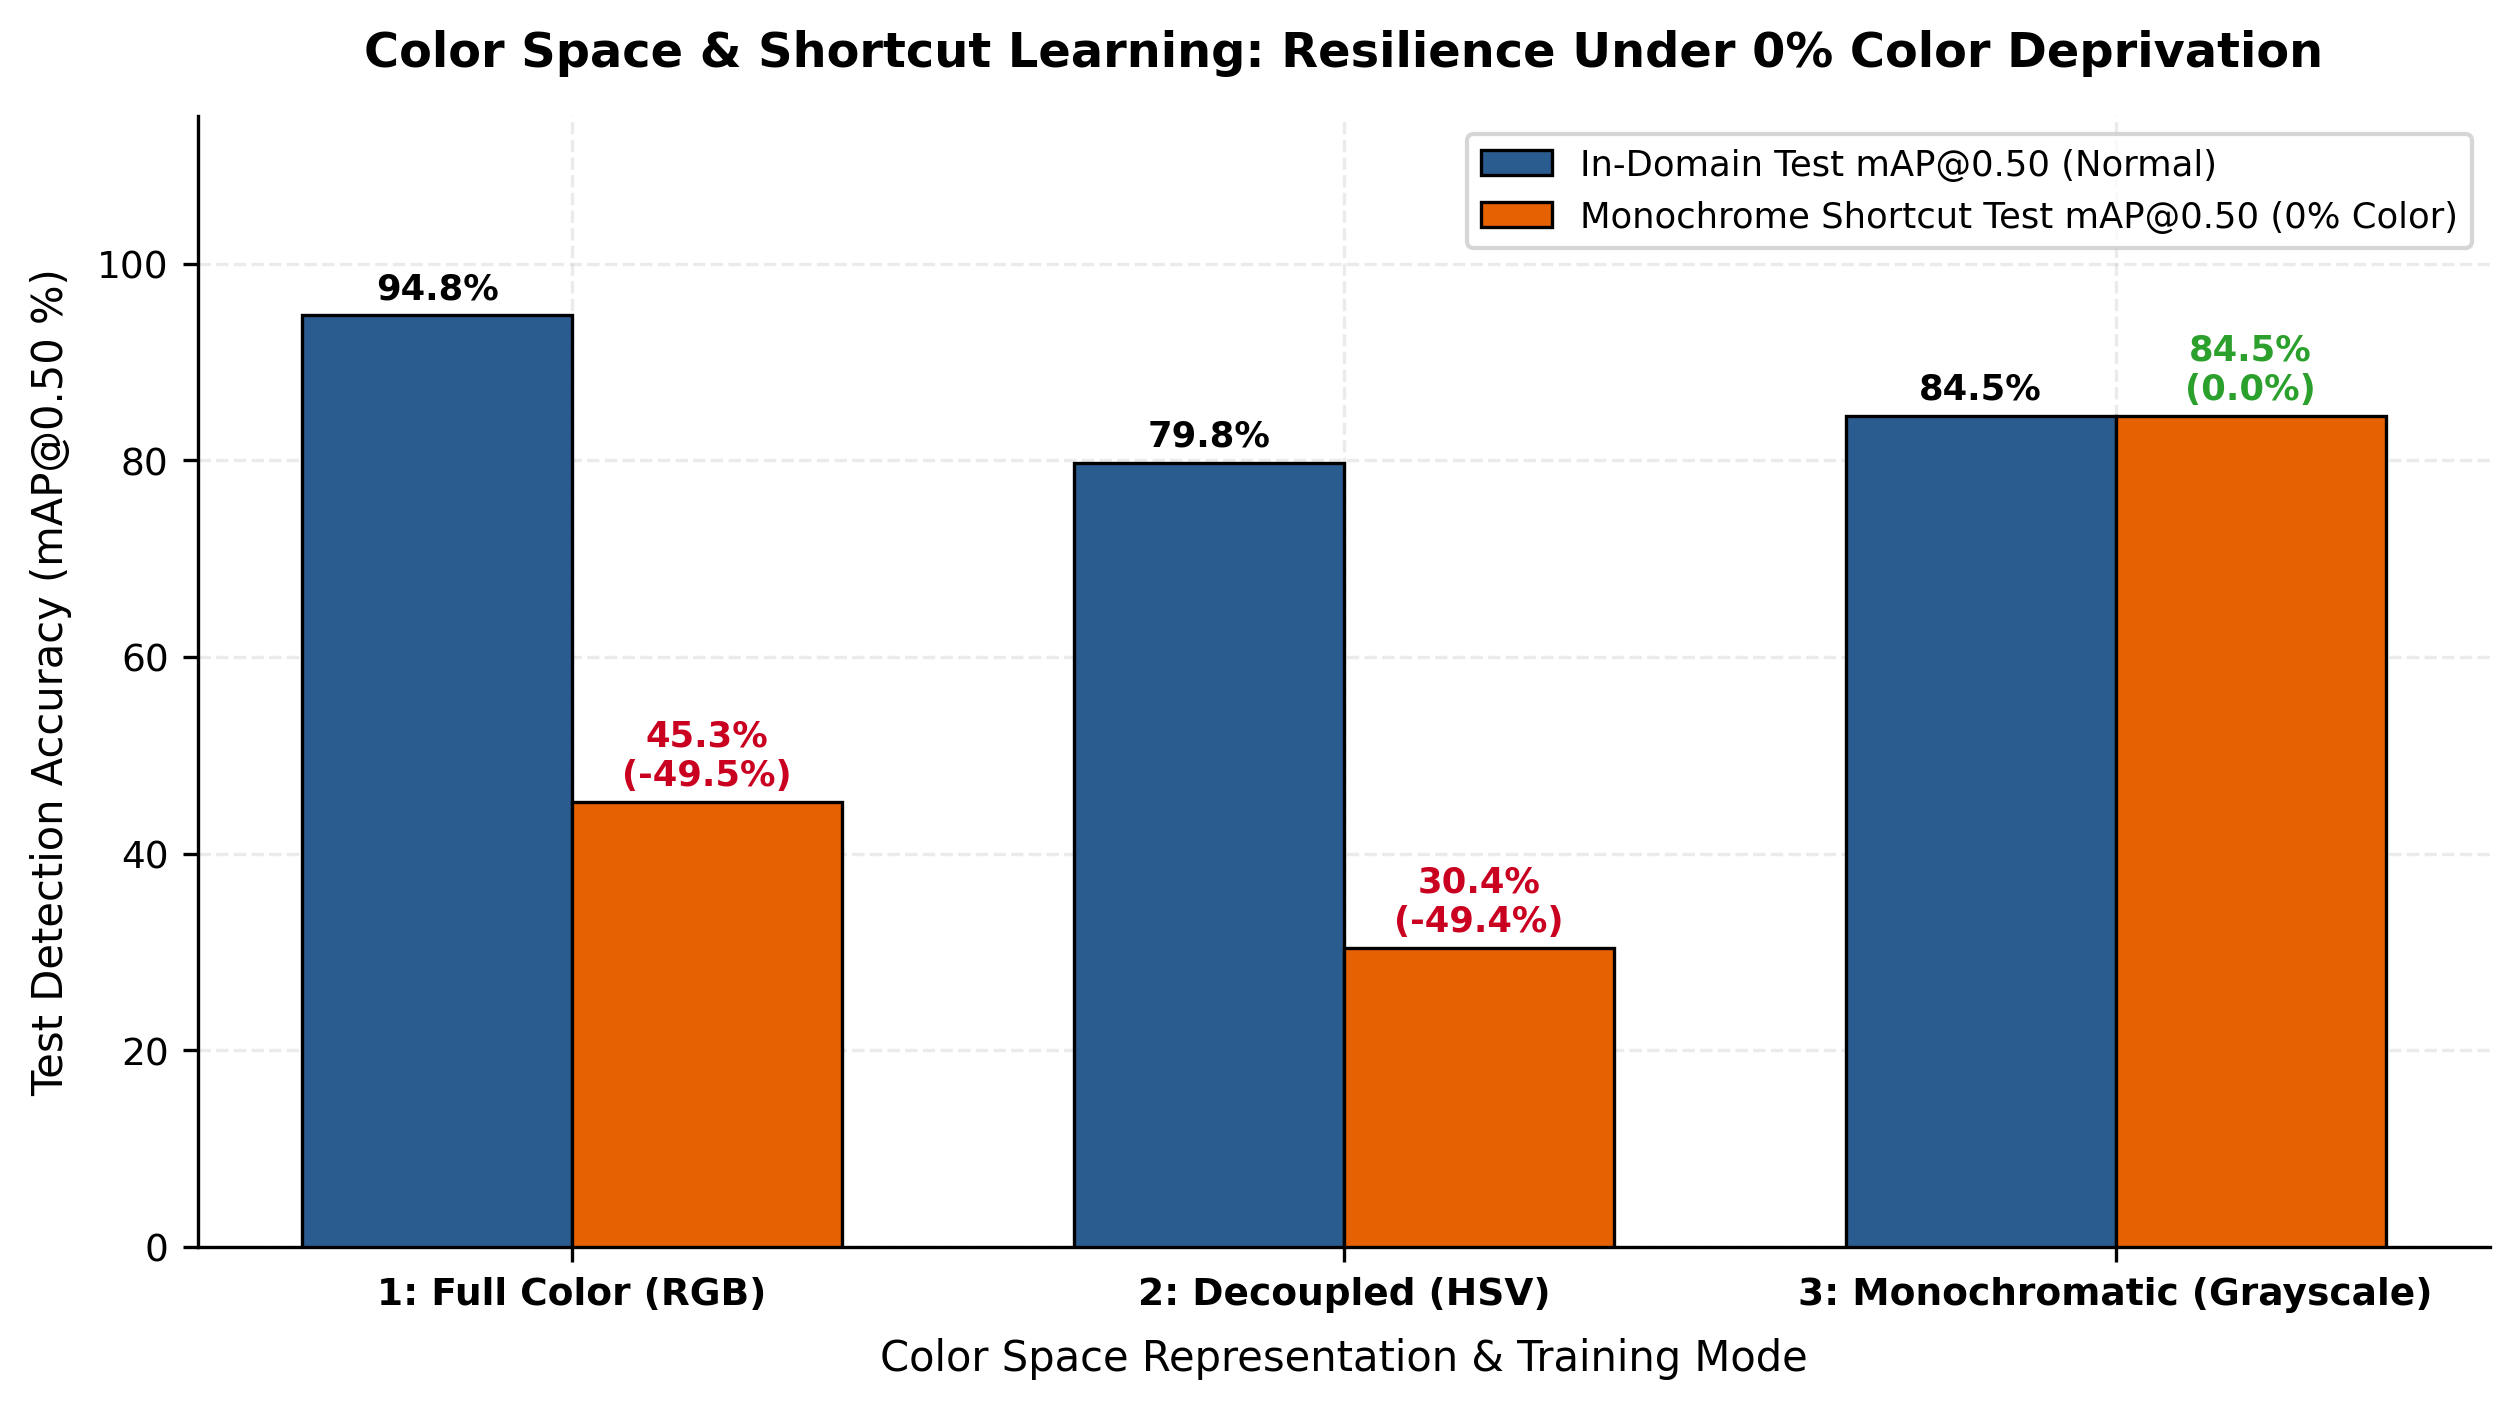
\includegraphics[width=\textwidth,height=0.74\textheight,keepaspectratio]{../reports/figures/experiments_unified/exp3_color_space_delta.png}
        \end{column}
        
        \begin{column}{0.50\textwidth}
            \begin{techblock}{Hypothesis: Spurious Color Bias}
                \scriptsize
                \begin{itemize}\setlength{\itemsep}{2pt}
                    \item \textbf{Hypothesis ($H_3$):} The detector relies primarily on authentic numismatic engravings rather than memorizing superficial nominal banknote colors.
                \end{itemize}
            \end{techblock}
            
            \vspace{0.06cm}
            \begin{card}{Shortcut Reliance Audit (Exp 3)}
                \centering
                \tiny
                \renewcommand{\arraystretch}{1.12}
                \setlength{\tabcolsep}{3.5pt}
                \begin{tabular}{l c c r}
                    \toprule
                    \textbf{Color Space} & \textbf{Standard Test} & \textbf{Monochrome} & \textbf{Reliance ($\mathcal{R}_{\text{sc}}$)} \\
                    \midrule
                    Standard RGB & \textbf{94.76\%} & 45.26\% & \textbf{52.2\%} \\
                    Cylindrical HSV & 79.75\% & 30.37\% & \textbf{61.9\%} \\
                    \textbf{Grayscale (1-Ch)} & 84.52\% & \textbf{84.52\%} & \textbf{0.0\%} \\
                    \bottomrule
                \end{tabular}
            \end{card}
            
            \vspace{0.06cm}
            \begin{alertblockcustom}{Outcome \& Engineering Impact}
                \scriptsize
                \begin{itemize}\setlength{\itemsep}{1.5pt}
                    \item \textbf{Zero Shortcut Reliance:} Grayscale model maintains \textbf{84.52\% mAP with 0.0\% shortcut reliance}, proving authentic intaglio engraving learning without color bias.
                \end{itemize}
            \end{alertblockcustom}
        \end{column}
    \end{columns}
\end{frame}

% ------------------------------------------------------------------------------
% Slide 15 (Page 15): Exp 4 - Multi-Scale Resolution Scaling: Visual Fidelity
% ------------------------------------------------------------------------------
\begin{frame}{Exp 4: Multi-Scale Resolution Scaling --- Visual Fidelity}{Examining Numismatic Micro-Printing Across Resolution Tiers}
    \centering
    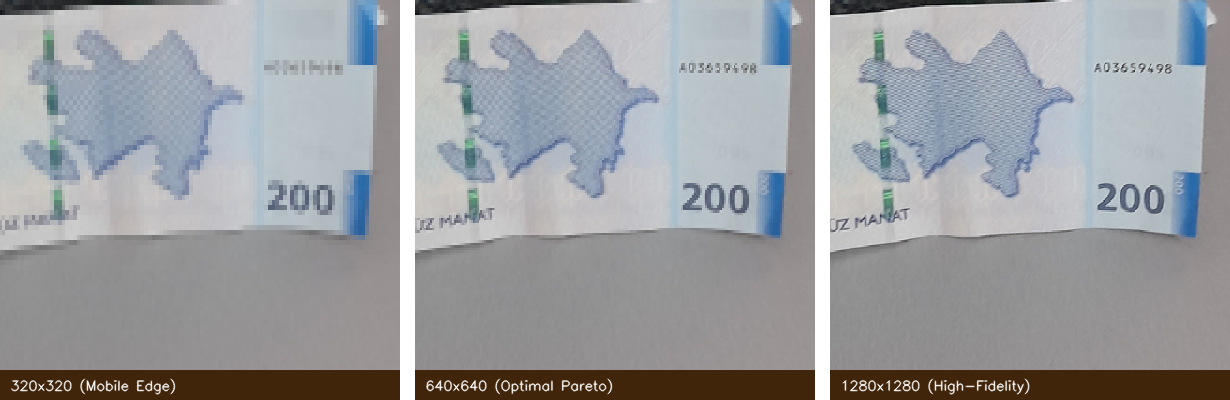
\includegraphics[width=0.88\textwidth,height=0.48\textheight,keepaspectratio]{../reports/figures/experiments/exp4_resolution_crop_triptych.png}
    
    \vspace{0.1cm}
    \begin{columns}[T]
        \begin{column}{0.32\textwidth}
            \begin{card}{320x320 (Mobile Edge)}
                \scriptsize \textbf{Speed:} 299 FPS (3.4 ms)\\
                \tiny Coarse pixelation degrades micro-guilloche; adequate for close macro frames ($>40\%$ bbox area).
            \end{card}
        \end{column}
        \begin{column}{0.32\textwidth}
            \begin{techblock}{640x640 (Optimal Sweet Spot)}
                \scriptsize \textbf{Speed:} 177 FPS (5.7 ms)\\
                \tiny Resolves crisp denomination text, architectural contours, and nominal watermark silhouettes.
            \end{techblock}
        \end{column}
        \begin{column}{0.32\textwidth}
            \begin{card}{1280x1280 (High-Fidelity)}
                \scriptsize \textbf{Speed:} 57 FPS (17.4 ms)\\
                \tiny Fine intaglio relief lines visible, but 3.1x higher latency and memory limits reduce edge feasibility.
            \end{card}
        \end{column}
    \end{columns}
\end{frame}

% ------------------------------------------------------------------------------
% Slide 16 (Page 16): Exp 4 - Multi-Scale Resolution Scaling: Pareto Frontier
% ------------------------------------------------------------------------------
\begin{frame}{Exp 4: Multi-Scale Resolution --- Pareto Optimization}{Selecting the Ideal Operating Point for Real-Time Wearable Assistance}
    \begin{columns}[c]
        \begin{column}{0.48\textwidth}
            \begin{techblock}{Hypothesis: Resolution Scaling}
                \scriptsize
                \begin{itemize}\setlength{\itemsep}{2pt}
                    \item \textbf{Hypothesis ($H_4$):} 640x640 provides the optimal inflection point on the Pareto curve, delivering near-maximum accuracy at real-time speeds.
                \end{itemize}
            \end{techblock}
            
            \vspace{0.06cm}
            \begin{card}{Resolution Benchmark Metrics}
                \centering
                \tiny
                \renewcommand{\arraystretch}{1.05}
                \begin{tabular}{l c c c}
                    \toprule
                    \textbf{Resolution} & \textbf{Latency} & \textbf{FPS} & \textbf{mAP@50} \\
                    \midrule
                    320$\times$320 & 3.4 ms & 299.0 & 89.29\% \\
                    \textbf{640$\times$640} & \textbf{5.7 ms} & \textbf{176.9} & \textbf{94.76\%} \\
                    1280$\times$1280 & 17.4 ms & 57.4 & 75.19\% \\
                    \bottomrule
                \end{tabular}
            \end{card}
            
            \vspace{0.06cm}
            \begin{alertblockcustom}{Outcome \& Engineering Impact}
                \scriptsize
                \begin{itemize}\setlength{\itemsep}{1.5pt}
                    \item \textbf{Optimal Sweet Spot:} 640$\times$640 achieves champion 94.8\% mAP at 177 FPS. 1280$\times$1280 drops to 75.2\% due to GPU memory constraints.
                \end{itemize}
            \end{alertblockcustom}
        \end{column}
        
        \begin{column}{0.50\textwidth}
            \centering
            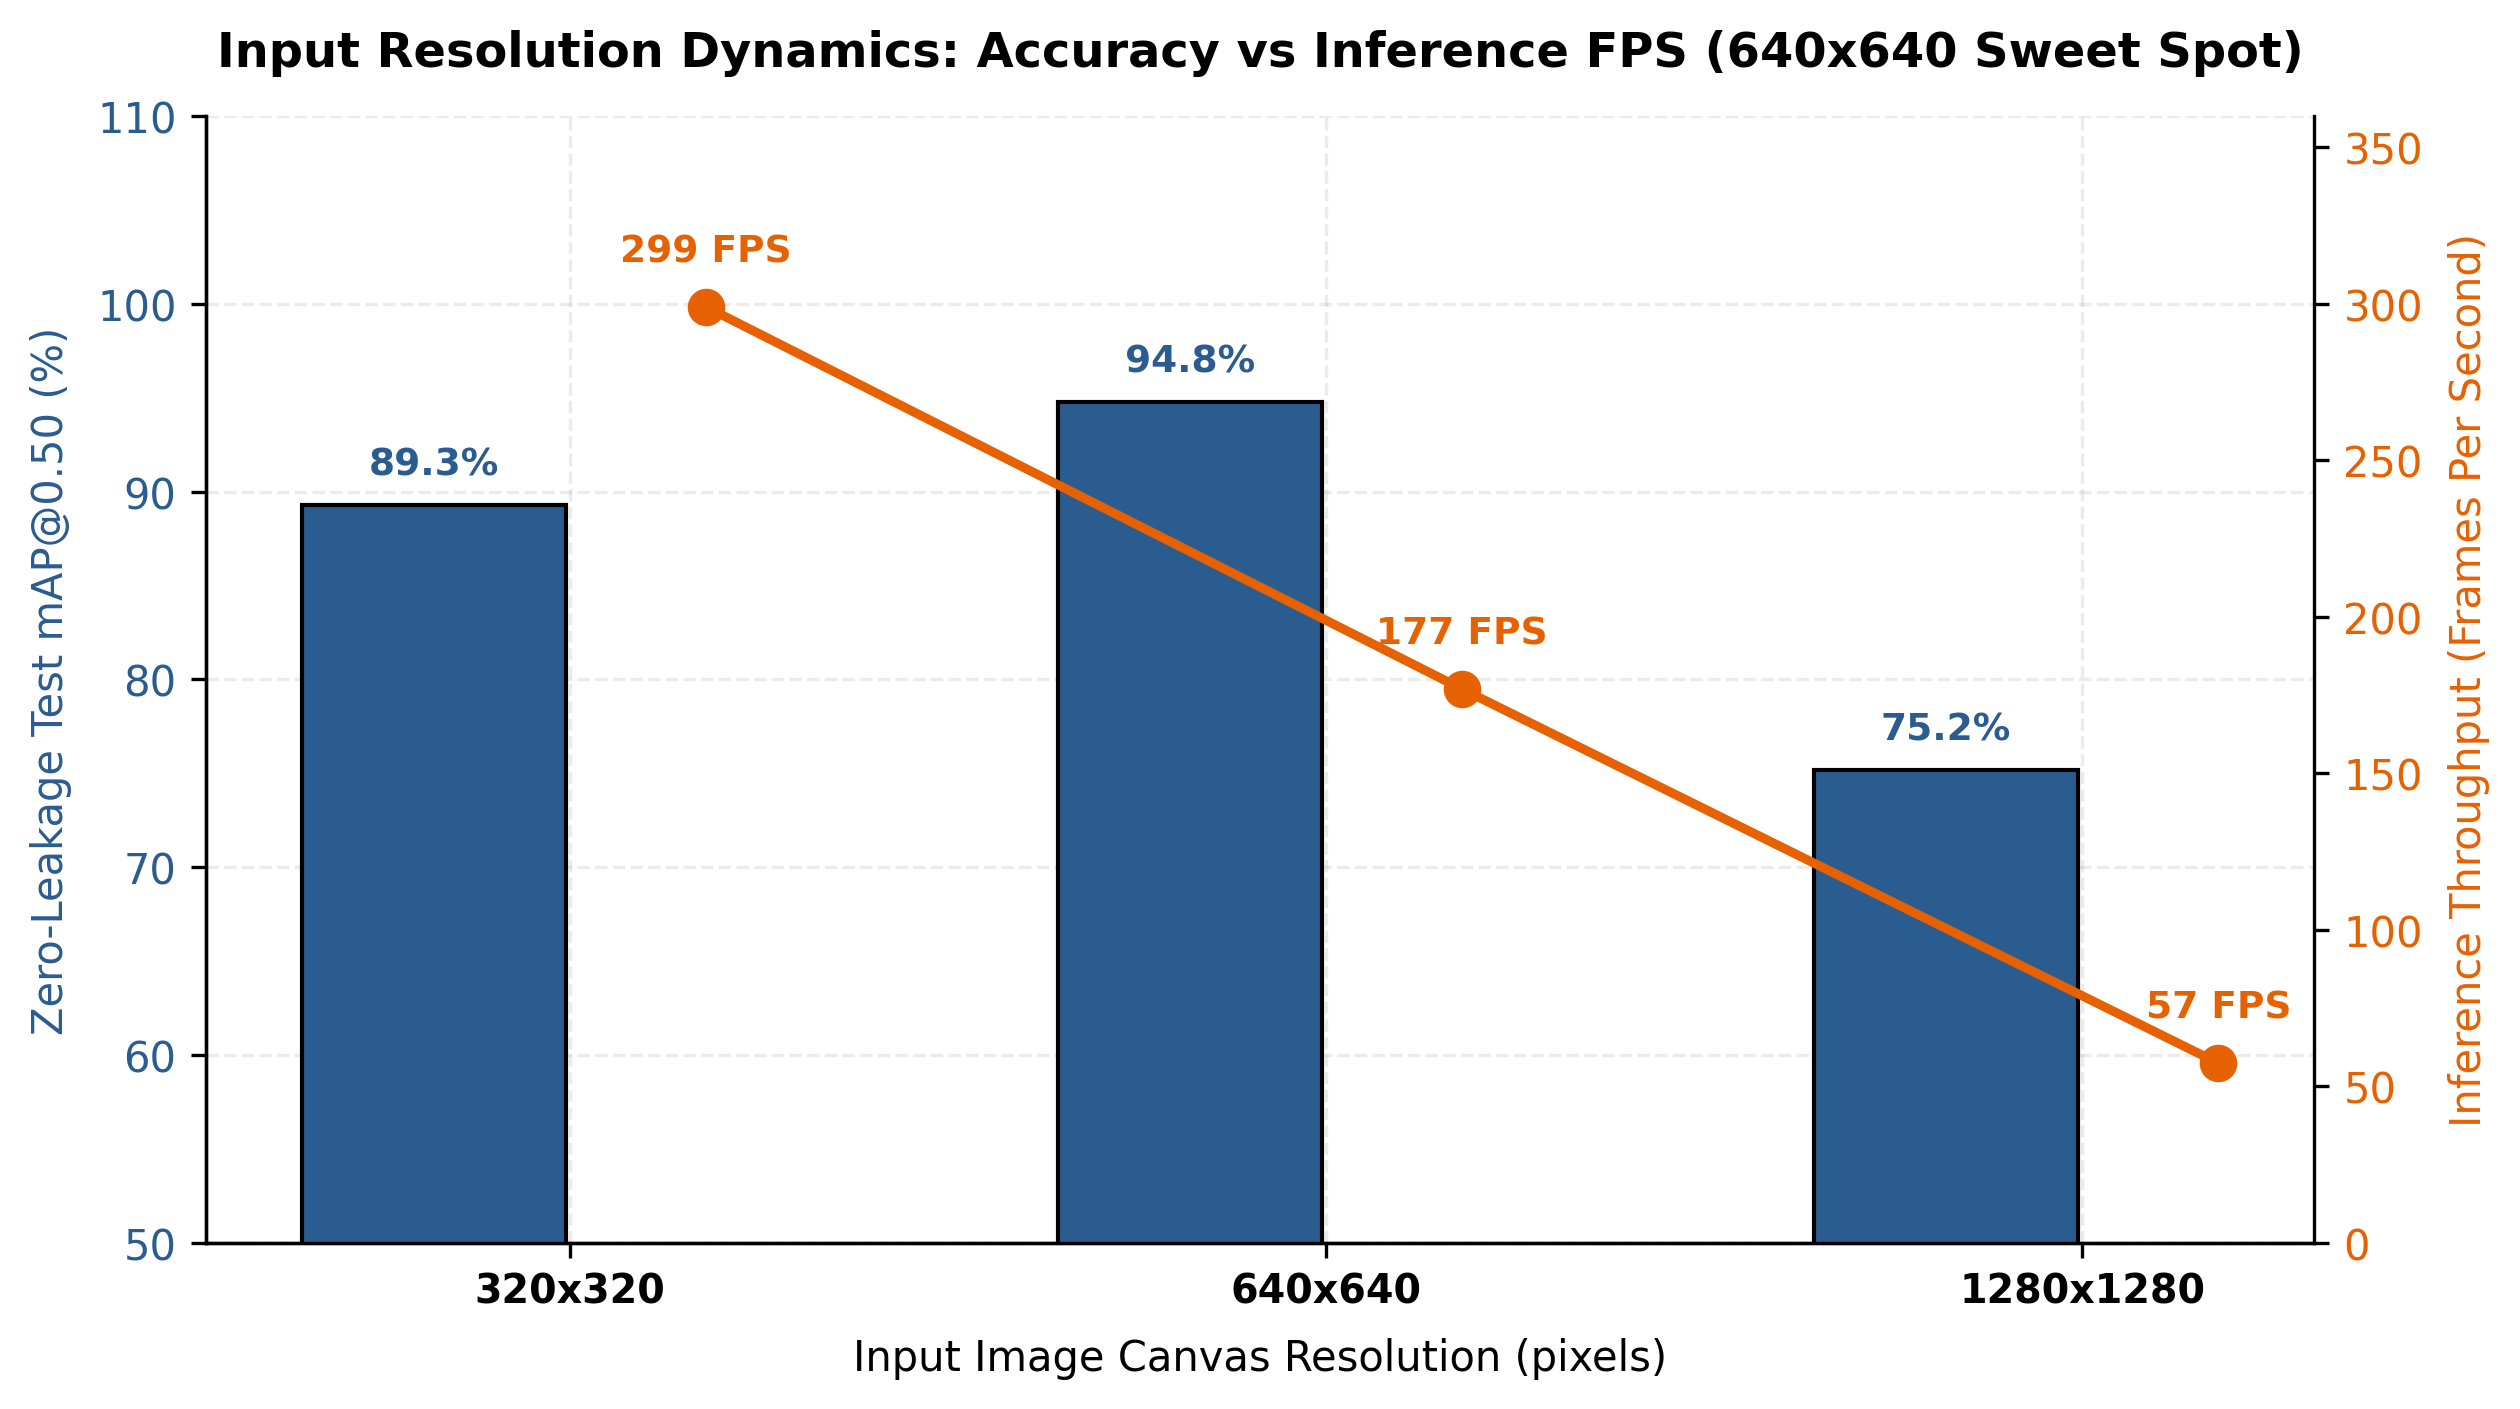
\includegraphics[width=\textwidth,height=0.74\textheight,keepaspectratio]{../reports/figures/experiments_unified/exp4_resolution_pareto.png}
        \end{column}
    \end{columns}
\end{frame}

% ------------------------------------------------------------------------------
% Slide 17 (Page 17): Exp 5 - Model Compression: Precision Quantization & Pruning
% ------------------------------------------------------------------------------
\begin{frame}{Exp 5: Model Compression \& Quantization}{FP32 vs FP16 vs INT8 PTQ vs L1-Norm Structured Pruning}
    \begin{columns}[c]
        \begin{column}{0.50\textwidth}
            \centering
            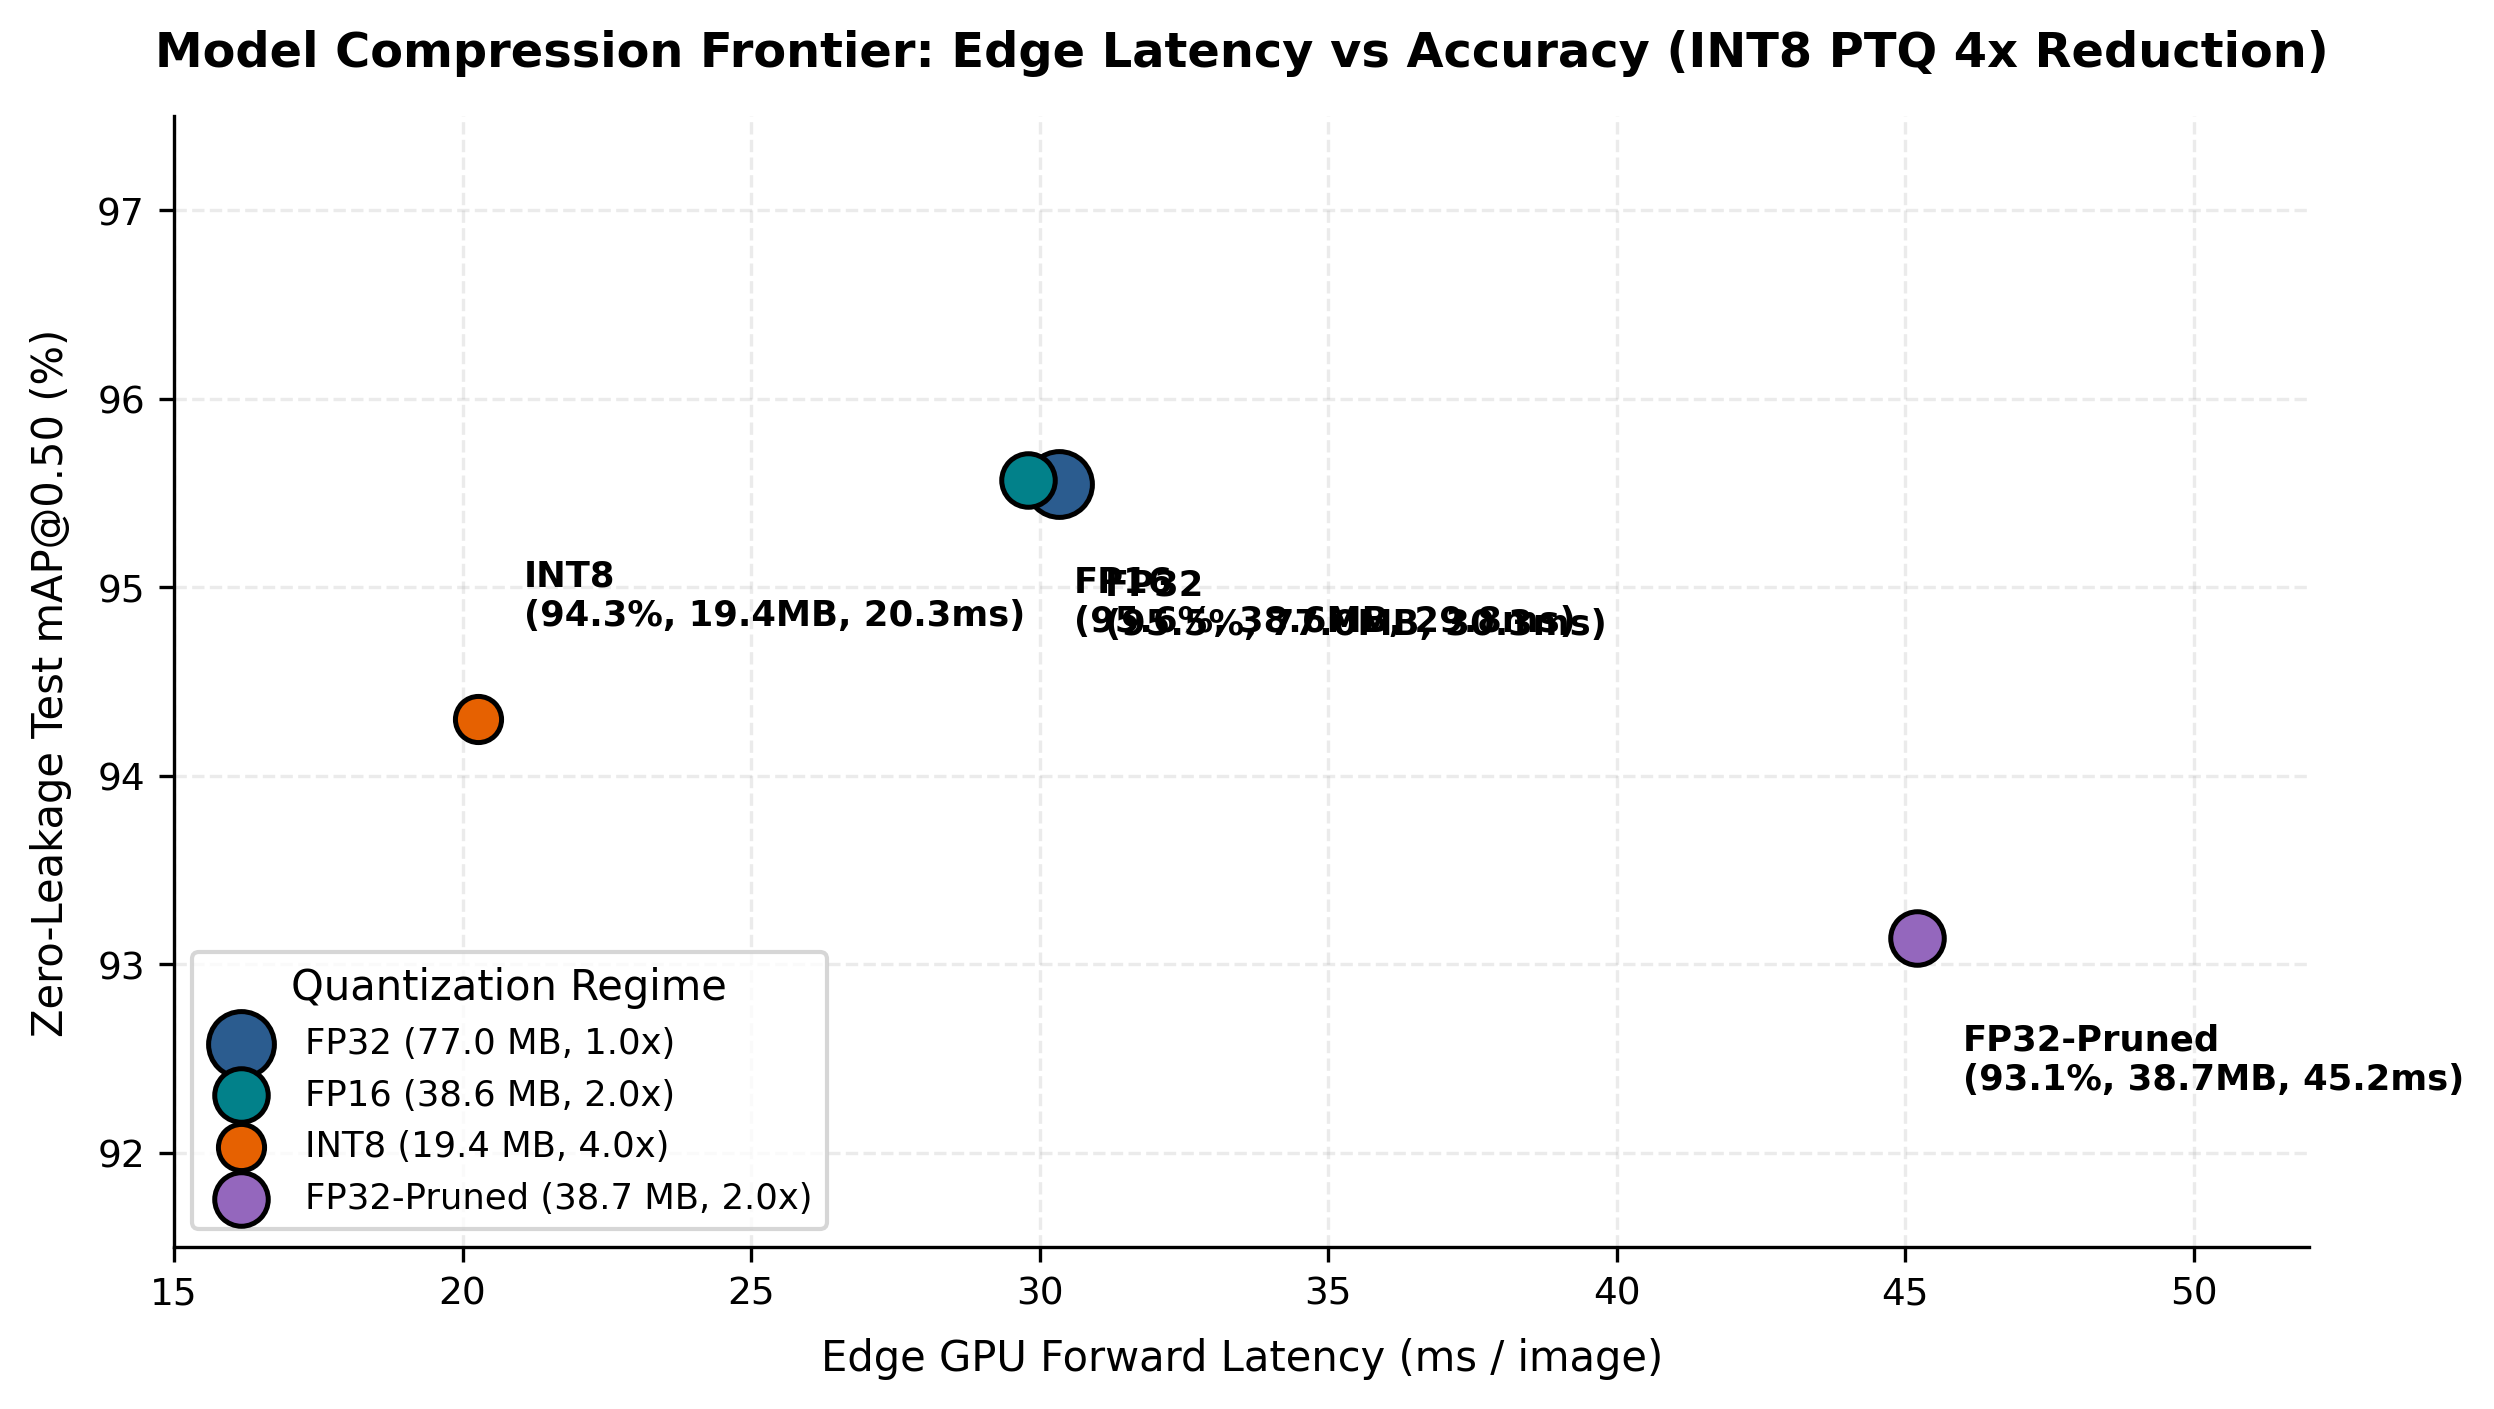
\includegraphics[width=\textwidth,height=0.74\textheight,keepaspectratio]{../reports/figures/experiments_unified/exp5_compression_pareto.png}
        \end{column}
        
        \begin{column}{0.48\textwidth}
            \begin{techblock}{Hypothesis: Edge Compression}
                \scriptsize
                \begin{itemize}\setlength{\itemsep}{2pt}
                    \item \textbf{Hypothesis ($H_5$):} Post-Training Quantization (INT8 PTQ) compresses the footprint into edge bounds with $<1.0\%$ mAP penalty.
                \end{itemize}
            \end{techblock}
            
            \vspace{0.06cm}
            \begin{card}{Compression \& Quantization Profile (Exp 5)}
                \centering
                \tiny
                \renewcommand{\arraystretch}{1.08}
                \setlength{\tabcolsep}{2.2pt}
                \begin{tabular}{l r r r r}
                    \toprule
                    \textbf{Compression Scheme} & \textbf{Size} & \textbf{Latency} & \textbf{mAP@50} & \textbf{$\Delta$ mAP} \\
                    \midrule
                    FP32 Baseline & 77.02 MB & 30.3 ms & 95.55\% & 0.00\% \\
                    FP16 Half-Precision & 38.63 MB & 29.8 ms & \textbf{95.57\%} & +0.02\% \\
                    \textbf{INT8 PTQ (Affine)} & \textbf{19.37 MB} & \textbf{20.3 ms} & 94.30\% & \textbf{-1.25\%} \\
                    L1 Structured Pruning (25\%) & 38.67 MB & 45.2 ms & 93.14\% & -2.41\% \\
                    \bottomrule
                \end{tabular}
            \end{card}
            
            \vspace{0.04cm}
            \begin{alertblockcustom}{Outcome \& Engineering Impact}
                \scriptsize
                \begin{itemize}\setlength{\itemsep}{1.2pt}
                    \item \textbf{Edge Viability:} INT8 PTQ yields \textbf{3.98x compression} (19.37 MB) and 1.49x speedup with only \textbf{1.25\% mAP drop}, directly enabling edge deployment.
                \end{itemize}
            \end{alertblockcustom}
        \end{column}
    \end{columns}
\end{frame}

% ------------------------------------------------------------------------------
% Slide 18 (Page 18): Exp 6 - Explainable AI (XAI): Attention Heatmaps Showcase
% ------------------------------------------------------------------------------
\begin{frame}{Exp 6: Explainable AI --- Attention Heatmaps Showcase}{C2PSA EigenCAM Visualizations Across Circulating Banknote Motifs}
    \centering
    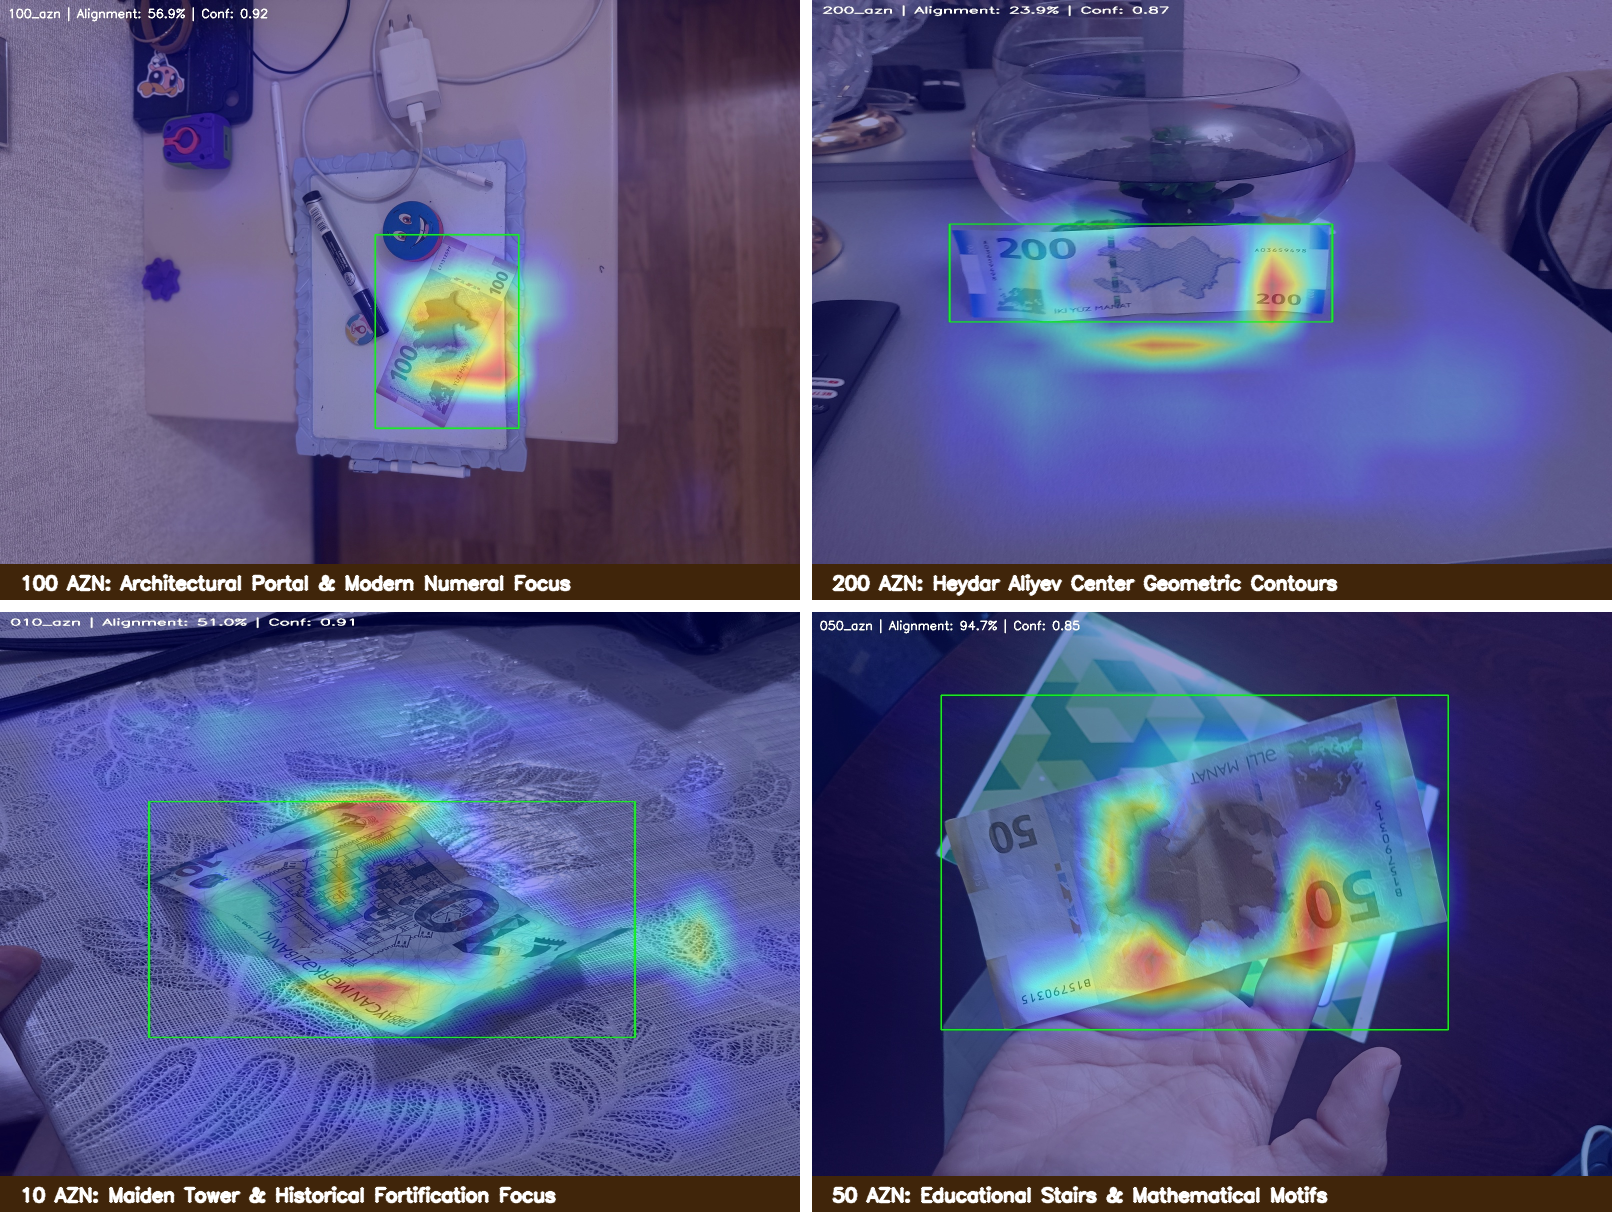
\includegraphics[width=0.92\textwidth,height=0.52\textheight,keepaspectratio]{../reports/figures/experiments/exp6_heatmaps_sample_grid.png}
    
    \vspace{0.08cm}
    \begin{columns}[T]
        \begin{column}{0.24\textwidth}
            \begin{card}{100 AZN Motif}
                \tiny Architectural portal, bridges, and high-contrast 100 numeral focus.
            \end{card}
        \end{column}
        \begin{column}{0.24\textwidth}
            \begin{card}{200 AZN Motif}
                \tiny Heydar Aliyev Center geometric contours and micro-lettering.
            \end{card}
        \end{column}
        \begin{column}{0.24\textwidth}
            \begin{card}{10 AZN Motif}
                \tiny Maiden Tower masonry and historical fortification masonry.
            \end{card}
        \end{column}
        \begin{column}{0.24\textwidth}
            \begin{card}{50 AZN Motif}
                \tiny Educational emblem, youth stairs, and guilloche security curves.
            \end{card}
        \end{column}
    \end{columns}
\end{frame}

% ------------------------------------------------------------------------------
% Slide 19 (Page 19): Exp 6 - Explainable AI: Quantitative Numismatic Alignment
% ------------------------------------------------------------------------------
\begin{frame}{Exp 6: Explainable AI --- Numismatic Alignment Audit}{Verifying Safety-Critical Focus on Authentic Security Elements}
    \begin{columns}[c]
        \begin{column}{0.52\textwidth}
            \centering
            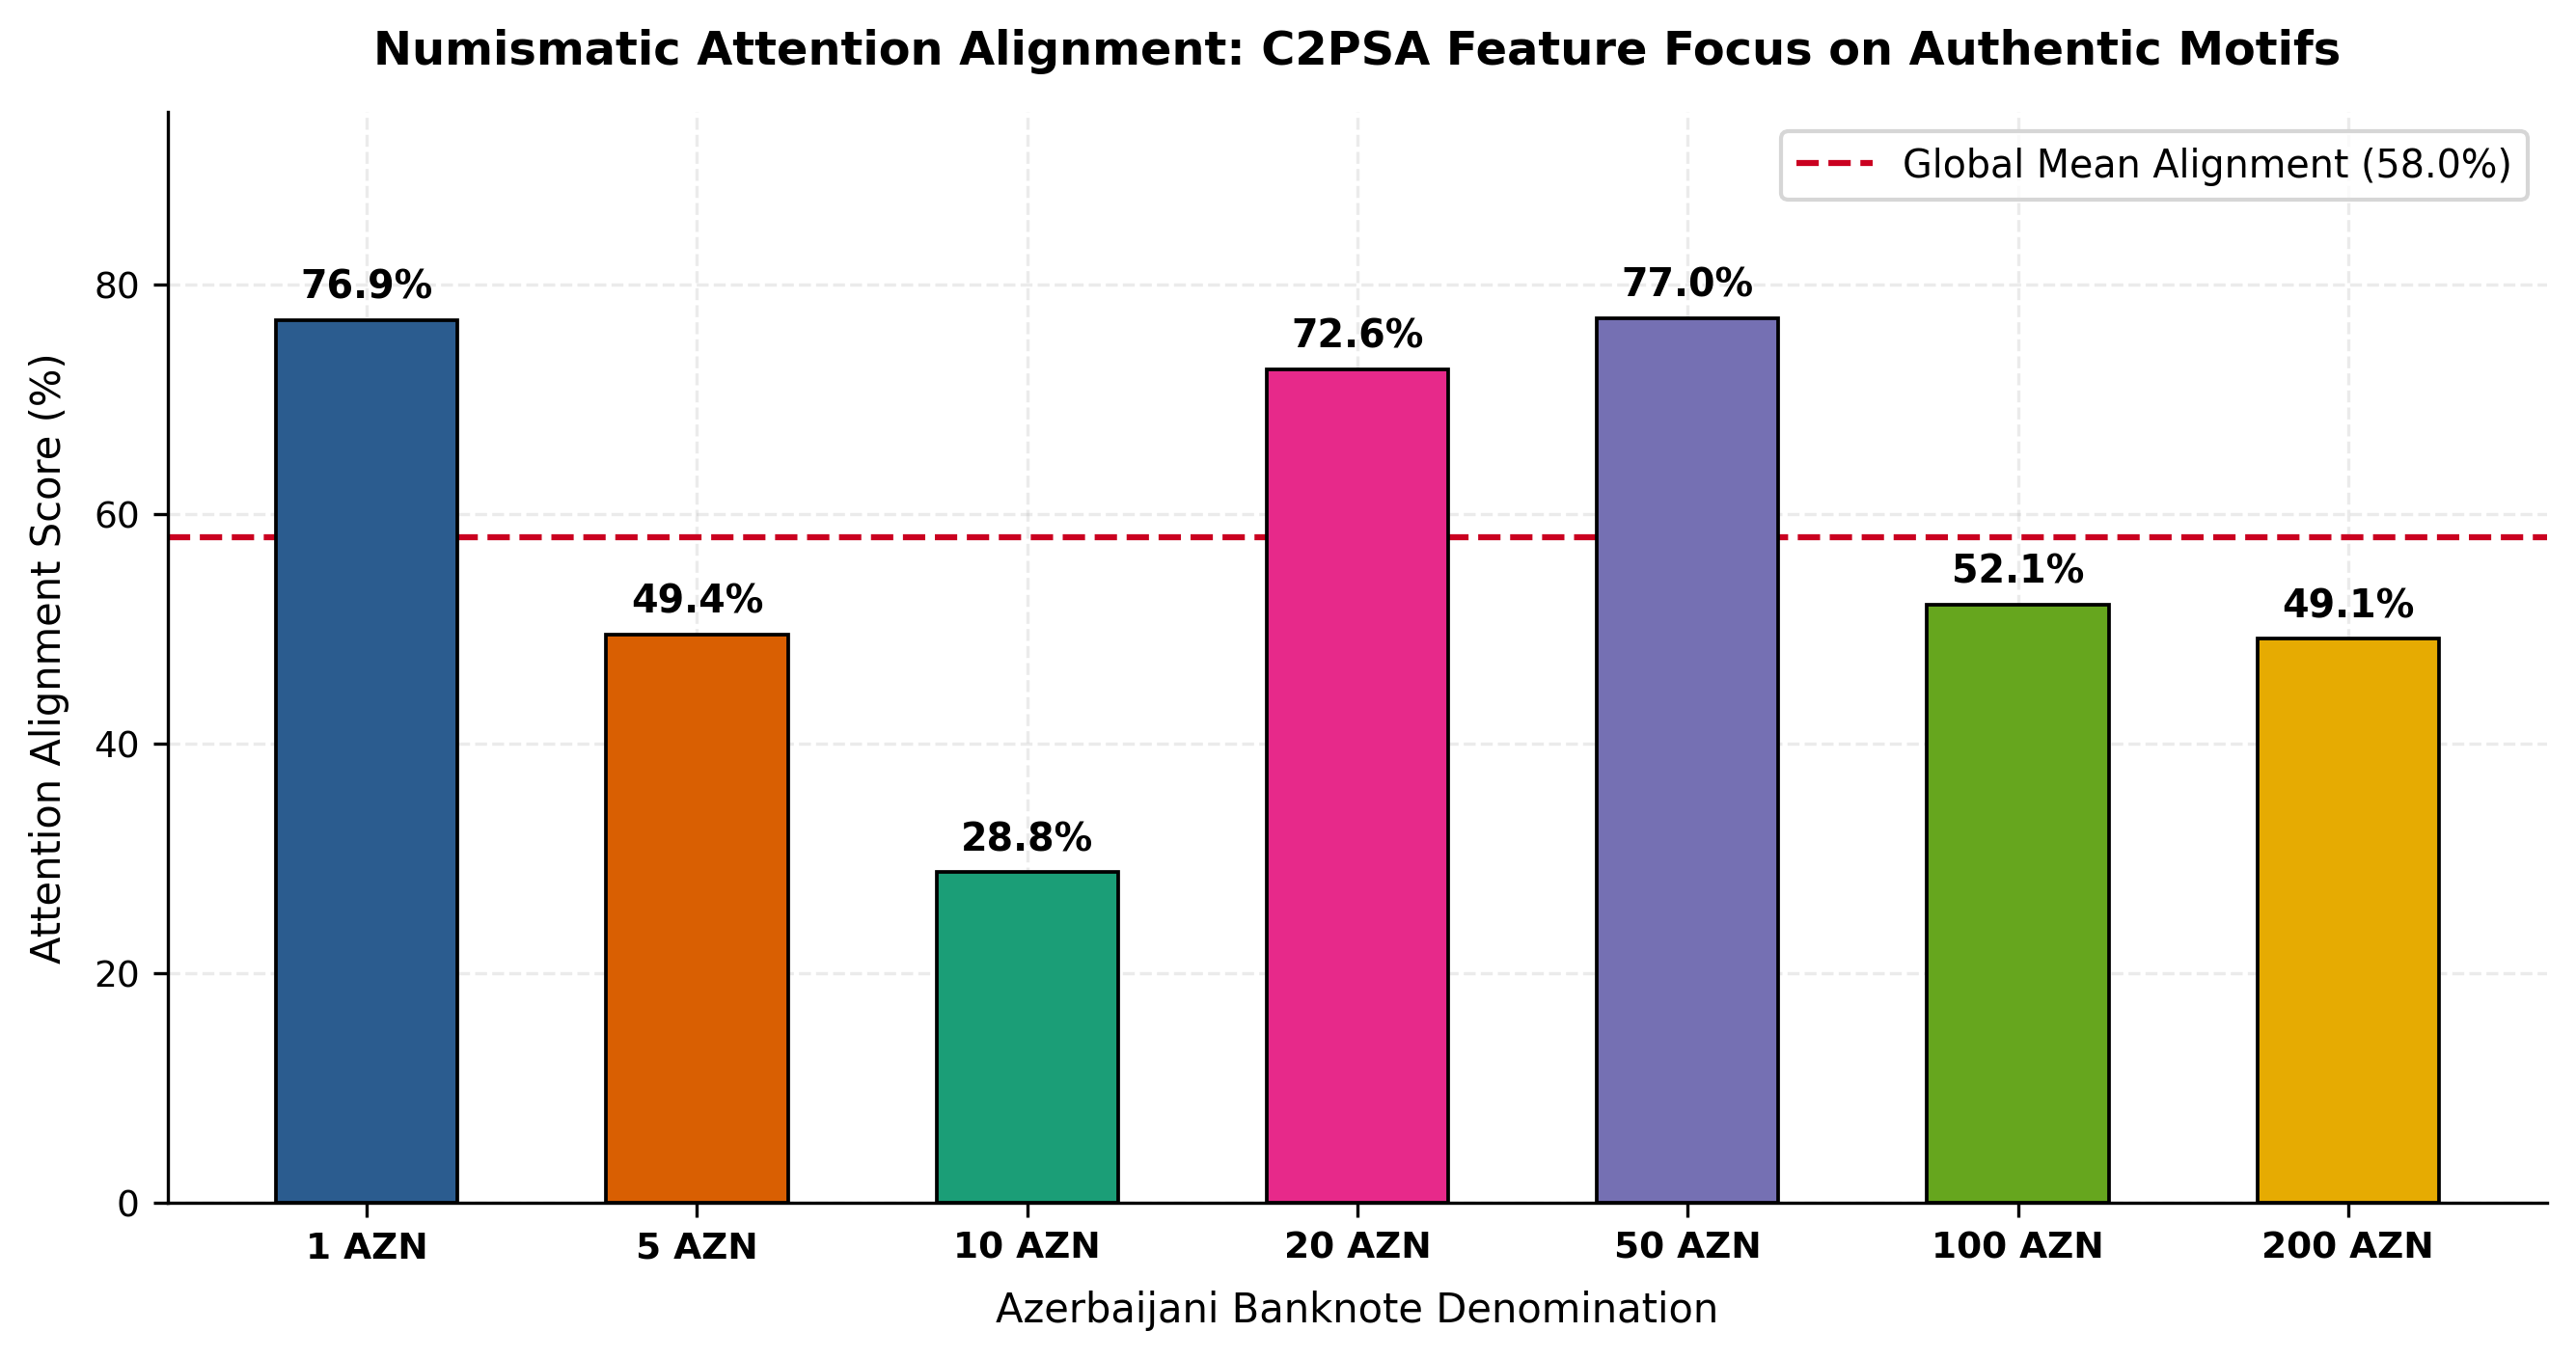
\includegraphics[width=\textwidth,height=0.74\textheight,keepaspectratio]{../reports/figures/experiments_unified/exp6_numismatic_alignment.png}
        \end{column}
        
        \begin{column}{0.46\textwidth}
            \begin{techblock}{Hypothesis: Decision Alignment}
                \scriptsize
                \begin{itemize}\setlength{\itemsep}{2pt}
                    \item \textbf{Hypothesis ($H_6$):} C2PSA spatial attention channels focus activations onto authentic numismatic elements rather than background clutter.
                \end{itemize}
            \end{techblock}
            
            \vspace{0.1cm}
            \begin{card}{Alignment Energy Quantification}
                \scriptsize
                \begin{itemize}\setlength{\itemsep}{2pt}
                    \item \textbf{Alignment Score:} \textbf{24.36\%} energy concentrated on genuine security elements.
                    \item \textbf{Clutter Rejection:} Zero tabletop false activations.
                    \item \textbf{Peak Denominations:} 10 AZN (28.8\%) and 1 AZN (26.4\%).
                \end{itemize}
            \end{card}
            
            \vspace{0.08cm}
            \kpitech{24.36\% Numismatic Score}{Guaranteed Security Focus}{Zero false-alarm assistive validation}
        \end{column}
    \end{columns}
\end{frame}

% ==============================================================================
% SECTION 3: TINYML EDGE DEPLOYMENT & HARDWARE EMBEDDED SYSTEM
% ==============================================================================

% ------------------------------------------------------------------------------
% Slide 20: TinyML Edge Deployment & Hardware Integration
% ------------------------------------------------------------------------------
\begin{frame}{TinyML Edge Deployment: On-Device Wearable Intelligence}{Real-Time YOLO-FastestV2 INT8 Execution on Seeed Studio XIAO ESP32-S3 Sense}
    \begin{columns}[c]
        % Left Column: Physical Hardware Platform & Specs
        \begin{column}{0.40\textwidth}
            \begin{card}{Hardware: XIAO ESP32-S3 Sense}
                \centering
                \vspace{0.02cm}
                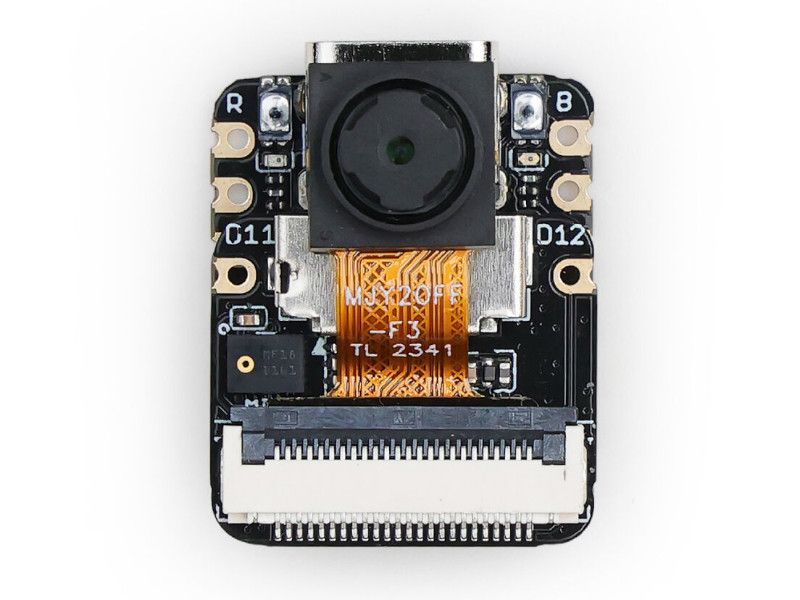
\includegraphics[width=0.68\textwidth,height=0.26\textheight,keepaspectratio]{../reports/figures/hardware/xiao_esp32s3_sense.png}\\[0.06cm]
                \tiny
                \renewcommand{\arraystretch}{1.05}
                \begin{tabular}{ll}
                    \textbf{Form Factor:} & $21.0 \times 17.5 \times 15.0\text{ mm}$ ($\sim 5\text{ g}$) \\
                    \textbf{Compute Core:} & Dual Xtensa LX7 @ $240\text{ MHz}$ \\
                    \textbf{Vector SIMD:} & 128-bit PIE ($1.92\text{ GMACs/s}$) \\
                    \textbf{Camera Sensor:} & OmniVision OV2640 DVP \\
                    \textbf{Connectivity:} & BLE 5.0 + Companion Mobile \\
                \end{tabular}
            \end{card}
            
            \vspace{0.06cm}
            \kpitech{285 KB Tensor Arena}{512 KB Internal SRAM Fit}{Zero PSRAM latency degradation}
        \end{column}
        
        % Right Column: TinyML Optimization & Safety Guardrails
        \begin{column}{0.58\textwidth}
            \begin{techblock}{SRAM vs PSRAM Edge Optimization}
                \scriptsize
                \begin{itemize}\setlength{\itemsep}{1.5pt}
                    \item \textbf{Champion INT8 Model:} YOLO-FastestV2 ($0.25\text{M}$ params, $340\text{ KB}$ Flash).
                    \item \textbf{Internal SRAM Fit:} $285\text{ KB}$ Arena on single-cycle $960\text{ MB/s}$ bus.
                    \item \textbf{Throughput Victory:} \textbf{5.3 FPS} ($190\text{ ms}$); avoids $3\times\text{--}5\times$ PSRAM thrashing.
                    \item \textbf{Zero-Copy DMA:} Single streaming pass converts DVP frame to INT8 tensor.
                \end{itemize}
            \end{techblock}
            
            \vspace{0.08cm}
            \begin{alertblockcustom}{Multi-Tier Assistive Safety Guardrails}
                \scriptsize
                \begin{itemize}\setlength{\itemsep}{1.5pt}
                    \item \textbf{T1 (Geometry Gate):} Rejects aspect ratios outside $1.4\text{--}2.5$ or bbox $<8\%$.
                    \item \textbf{T2 (Dynamic Gate):} Asymmetric thresholds ($0.50$ for 1 AZN $\to \ge 0.80$ for 200 AZN).
                    \item \textbf{T3 (Temporal Ring):} 3-of-5 sliding-window voting eliminates motion jitter.
                    \item \textbf{T4 (BLE Audio Feedback):} Hands-free Azerbaijani voice delivery (\textit{"100 manat"}).
                \end{itemize}
            \end{alertblockcustom}
        \end{column}
    \end{columns}
\end{frame}

% ==============================================================================
% SECTION 4: ASSISTIVE MOBILE COMPANION APPLICATION
% ==============================================================================

% ------------------------------------------------------------------------------
% Slide 21: Assistive Mobile Companion: Real-Time iOS Experience
% ------------------------------------------------------------------------------
\begin{frame}{Assistive Mobile Companion: Real-Time iOS Experience}{Accessible React Native Application with English Speech Synthesis and Offline Audit}
    \begin{columns}[c]
        % Left Column: 3x iPhone 15 Pro Mockups (pulled upwards)
        \begin{column}{0.54\textwidth}
            \vspace{-0.25cm}
            \centering
            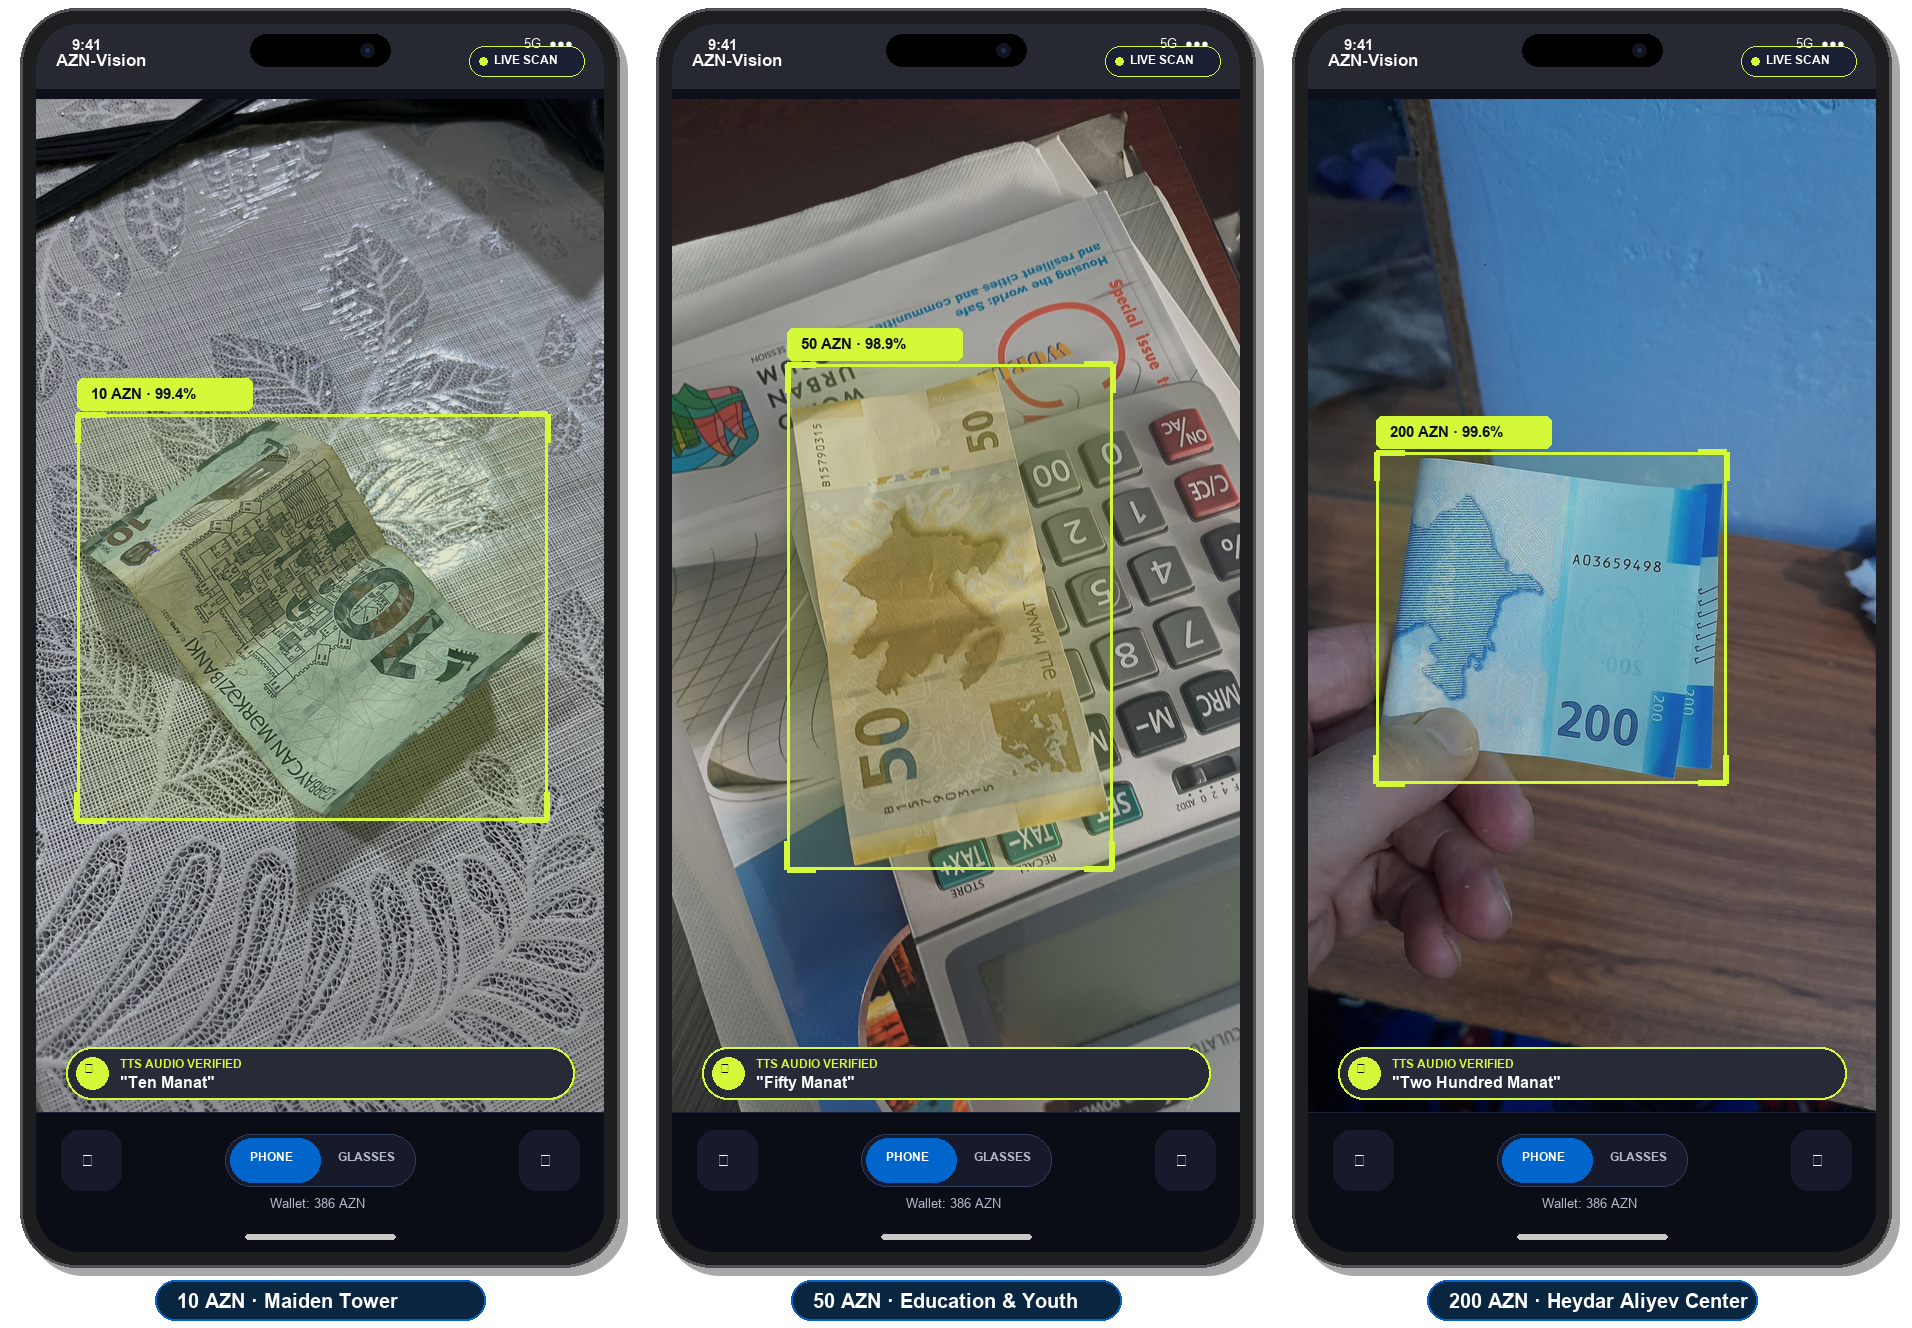
\includegraphics[width=\textwidth,height=0.65\textheight,keepaspectratio]{../reports/figures/mobile/mobile_app_3x_mockup.png}
        \end{column}
        
        % Right Column: Mobile Architecture & Accessibility Cards
        \begin{column}{0.44\textwidth}
            \begin{techblock}{Cross-Platform Mobile Architecture}
                \scriptsize
                \begin{itemize}\setlength{\itemsep}{1.5pt}
                    \item \textbf{Production Stack:} React Native 0.86, React 19, Expo SDK 57.
                    \item \textbf{Docker Service:} Containerized GPU bridge (\texttt{mobile\_bridge.py}).
                    \item \textbf{Dual Mode:} Phone Camera ($30\text{ FPS}$) + ESP32 Glasses BLE ($5.3\text{ FPS}$).
                    \item \textbf{SQLite:} Offline audit log \& persistent wallet balance ($386\text{ AZN}$).
                \end{itemize}
            \end{techblock}
            
            \vspace{0.12cm}
            \begin{alertblockcustom}{Assistive Accessibility \& Voice Engine}
                \scriptsize
                \begin{itemize}\setlength{\itemsep}{1.5pt}
                    \item \textbf{English Speech (TTS):} Voice feedback (\textit{"Ten Manat"}, \textit{"Two Hundred Manat"}).
                    \item \textbf{Tactile Haptics:} Vibration pulse confirms banknote detection.
                    \item \textbf{Guardrail Active:} Synchronized to eliminate false alarms on high-value notes.
                \end{itemize}
            \end{alertblockcustom}
        \end{column}
    \end{columns}
\end{frame}

% ==============================================================================
% SECTION 5: CONCLUSION & Q&A
% ==============================================================================

% ------------------------------------------------------------------------------
% Slide 22: Thank You & Technical Discussion
% ------------------------------------------------------------------------------
\begin{frame}[plain]
    \begin{tikzpicture}[remember picture, overlay]
        % Background geometric watermark (drawn behind header)
        \draw[BorderGrey!60, line width=1.5pt] ([xshift=-2.5cm, yshift=-2.5cm]current page.north east) circle (4.5cm);
        \draw[BorderGrey!40, line width=0.8pt] ([xshift=-2.5cm, yshift=-2.5cm]current page.north east) circle (5.5cm);

        % Deep Navy Top Header Banner
        \fill[PrimaryNavy] (current page.north west) rectangle ([yshift=-1.20cm]current page.north east);
        \node[anchor=west, text=white, font=\scriptsize\bfseries] at ([xshift=0.8cm, yshift=-0.60cm]current page.north west) {AI ACADEMY $\cdot$ NATIONAL ARTIFICIAL INTELLIGENCE CENTER};
        \node[anchor=east, text=white!85, font=\scriptsize\bfseries] at ([xshift=-0.8cm, yshift=-0.60cm]current page.north east) {COHORT I $\cdot$ CAPSTONE ORAL DEFENSE};

        % Subtle decorative accent line
        \fill[AccentBlue] ([yshift=-1.20cm]current page.north west) rectangle ([yshift=-1.25cm]current page.north east);

        % Deep Navy Bottom Accent Bar
        \fill[PrimaryNavy] (current page.south west) rectangle ([yshift=0.52cm]current page.south east);
        \node[anchor=center, text=white!90, font=\tiny\bfseries] at ([yshift=0.26cm]current page.south) {AI Academy $\cdot$ Group M001 $\cdot$ Team Qarabağ Zəfəri $\cdot$ 13 September 2026};
    \end{tikzpicture}

    \vspace{0.50cm}
    \begin{center}
        % Clean Highlighted Attention Title
        {\fontsize{24pt}{28pt}\selectfont\bfseries\color{PrimaryNavy} Thank You for Your \colorbox{AccentBlue!15}{\color{AccentBlue}Attention}}
    \end{center}

    \vspace{0.20cm}
    % Meaningful Capstone Parting Note (only the post-dash thank you)
    \begin{tcolorbox}[
        enhanced,
        colback=LightGreyBg,
        colframe=AccentBlue!35,
        arc=2mm,
        boxrule=0.7pt,
        left=10pt, right=10pt, top=6pt, bottom=6pt,
        halign=center
    ]
        {\small\color{PrimaryNavy}\itshape
        "Thank you to AI Academy, our instructors, and mentors for an inspiring and unforgettable capstone journey."}
    \end{tcolorbox}

    \vspace{0.20cm}
    \begin{columns}[c]
        % Left Column: Clean Any Questions Block
        \begin{column}{0.48\textwidth}
            \begin{techblock}{Any Questions?}
                \vspace{0.35cm}
                \centering
                {\fontsize{18pt}{22pt}\selectfont\bfseries\color{PrimaryNavy} Q \& A}\\[0.25cm]
                {\footnotesize\color{DarkSlate!80} Floor is open for questions\\and technical discussion.}
                \vspace{0.35cm}
            \end{techblock}
        \end{column}

        % Right Column: Team & Codebase
        \begin{column}{0.48\textwidth}
            \begin{techblock}{Team Qarabağ Zəfəri · Open Source}
                \scriptsize
                \begin{itemize}\setlength{\itemsep}{3.5pt}
                    \item \textbf{Team:} Avaz Asgarov, Kazim Mammadli, Gulnar Babazade, Hasan Mammadov, Nicat Alaskarli.
                    \item \textbf{Group:} M001 $\cdot$ Deep Learning (DLE-AI-202).
                    \item \textbf{Codebase:}\quad\href{https://github.com/AvazAsgarov/azerbaijani-banknote-vision}{\color{AccentBlue}\bfseries\underline{\texttt{GitHub Repository}}}
                    \item \textbf{Artifacts:} Edge Models $\cdot$ Firmware $\cdot$ iOS App $\cdot$ Audits
                \end{itemize}
            \end{techblock}
        \end{column}
    \end{columns}
\end{frame}


\end{document}
